\documentclass[conference]{IEEEtran}
\IEEEoverridecommandlockouts
% The preceding line is only needed to identify funding in the first footnote. If that is unneeded, please comment it out.

\usepackage{amsmath}
\usepackage{todonotes}
\usepackage{algorithm}
\usepackage[noend]{algpseudocode}
\usepackage{cite}
\usepackage{amsmath,amssymb,amsfonts}
\usepackage{algorithmic}
\usepackage{graphicx}
\usepackage{textcomp}
\usepackage{xcolor}
\def\BibTeX{{\rm B\kern-.05em{\sc i\kern-.025em b}\kern-.08em
    T\kern-.1667em\lower.7ex\hbox{E}\kern-.125emX}}
    
\usepackage{atbegshi}% http://ctan.org/pkg/atbegshi
\AtBeginDocument{\AtBeginShipoutNext{\AtBeginShipoutDiscard}}


\begin{document}

\title{ Application Note: $\mu$Polar \-- An Interactive 2D Visualization Tool for  Microfluidics and  Microscopic Time Series Images }

% \author{\IEEEauthorblockN{1\textsuperscript{st} Mehran Ghafari}
% \IEEEauthorblockA{\textit{SimCenter, Dept. Computer Science and Engineering} \\
% \textit{University of Tennessee, Chattanooga, USA}\\
% ryg668@mocs.utc.edu}
% \and
% \IEEEauthorblockN{2\textsuperscript{nd} Hao-Bo Guo}
% \IEEEauthorblockA{\textit{SimCenter, Dept. Computer Science and Engineering} \\
% \textit{University of Tennessee, Chattanooga, USA}\\
% haobo-guo03@utc.edu}
% \and
% \IEEEauthorblockN{3\textsuperscript{rd} Weiwei Dang}
% \IEEEauthorblockA{\textit{Dept. Molecular and Human Genetics, Huffington Center on Aging}\\
% \textit{Baylor College of Medicine, Houston, USA}\\
% Weiwei.Dang@bcm.edu}
% \and
% \IEEEauthorblockN{4\textsuperscript{th} Hong Qin}
% \IEEEauthorblockA{\textit{SimCenter, Dept. Computer Science and Engineering}\\
% {Dept. Biology, Geology and Enviromental Science} \\
% \textit{University of Tennessee, Chattanooga, USA}\\
% hong-qin@utc.edu}
% }

\maketitle


\begin{Summary}

Microfluidics-based microscopy is becoming an increasingly popular research tool to monitor cellular events in biomedical research. One such application is the high-throughput analysis of cells division. It is challenging to visualize and interpret the data gathered through microfluidics-based microscopy. Here, we developed a circular plotting method, $\mu$Polar, to visualize the cell movements and cellular division events at different time-points. Our method is interactive and easy to use. We demonstrated the utility of our method to describe the events of dividing yeast cells. Our method could be potentially applied to other types of microfluidic devices including microscopic images. This software is implemented in an R package $\mu$Polar\ available through GitHub.


\end{Summary}


\begin{IEEEkeywords}
Microfluidics devices, microscopic data, cell distance, $\mu$Polar visualization 
\end{IEEEkeywords}

\section{Introduction}
 
The biological processes of cell lineage family tree that deployed in spatial and temporal are essential in the biomedical field including research, medicine and diagnosis a variety of diseases. Thus, quantitative analysis of cell behavior constructed on lineage tree tagged with appropriate measurements for the individual cell is the imperative basis for understanding the dynamics and structure of organisms \cite{r2.6}. Comprehensive and detailed information considering cell locality position, pathway, nucleus, formation, dissection, replicative and chronological lifespan can potentially be concluded from images using a combination of manual and automatic visualization tools \cite{r2.7}. Having an automatic tool that collects microscopic images and generates interactive visualization of the cell family tree with a quantitative comparison of cells would be a great requisite for many applications.\\

In the recent decade, crucial breakthroughs have been created and developed in the microscopy imaging of live-cell mechanisms such as fluorescent protein labeling, selective plane illumination microscopy (SPIM) and multiphoton laser scanning microscopy (MLSM)\cite{r2.7,r2.8}. Concurrently, many image processing algorithms have been developed for cell segmentation (e.g, semantic and instance), tracking and quantitative analysis \cite{r2.10}.\\


Since many of the experimental results from microscopic images are based on numerical numbers which require expertise to verify the validation of the outcome, visualization can offer an efficient path to study data such as yeast cells biological data. However, it has not adequately been developed in time-lapse microscopic images with interactive visualization. In fact, there is a knowledgeable gap between some biology areas and suitable visualization tools, in particular, visualizing microfluidics images interpreting the dynamic development of cells and lifespan. 

Microfluidics device is an ultra-small structure with microfluid channels offer faster and reliable results in comparison to traditional methods \cite {r2.1,r2.2}. Duo to their functionality, microscale and nanoscale dimension, they can be used in many applications such as drug delivery, cell monitoring, cell division, virus inspection and so on \cite{r2.3,r2.4}. Time-lapse microfluidics images amplify biologists ability to experimentally image live-cell during the developing progress \cite{r3}. Recently, a new network model of cellular aging was proposed based on the cellular aging process of yeast cells \cite{ref4.2}. For instance, Jo et al. \cite{\r13} investigated the high-throughput analysis of dividing yeast cells using microfluidic devices.\\ 

Cell division enumeration is a budding yeast process considering one of the essential factors in the aging process where single mother cells can be accomplished before inactivation, also known as replicative lifespan (RLS). Determining the lifespan of cells is a time-consuming process and in many cases is based on manual operation, such as cell micro-dissection \cite{ref08}. Accordingly, visualization of cell growth and division potentially can offer a great point of view to estimate RLS of cells (e.g, yeast cells) which would have an effective impact in many applications. Hence, structural information in high-resolution is one of the essential factors in understanding the molecular dynamics and cell functionalities such microfluidics-based microscopy images. Yet, it is challenging to visualize and interpret the data gathered through microfluidics-based microscopy interactively.\\

To this end, we developed a circular plotting method, $\mu$Polar, to interpret cell movements and cellular division events at different time points from yeast cells microfluidics images. Our method is interactive and facile to utilize. We demonstrated the utility of our method to describe the events of dividing yeast cells over a time period. Our method could be potentially applied to other types of microfluidic devices including microscopic images.\\

The paper is organized as follows. In the results section, we concisely explain the data collection, feature extraction, and $\mu$Polar visualization analysis. In the discussion section, we focus on $\mu$Polar R package and $\mu$Polar functions. This section additionally covers some of $\mu$Polar plot examples including RLS. Finally, the conclusion section renders a summary of the proposed visualization method for microfluidics-based microscopic images.

 
%%%%%%%%%%%%%%%%%%%%%%%  to put note on pdf   %%%%%%%%%%%%%%%%%%%%%
%  One of the major \todo[inline]{change this to red}. However, ...
%%%%%%%%%%%%%%%%%%%%%%%%%%%%%%%%%%%%%%%%%%%%%%%%%%%%%%%%%%%%%%%%%%%


\section{Results}

We developed an R package called "$\mu$Polar" for time-lapse microfluidics-based microscopic images visualization where any individual image could be visualized based on the number of cells and areas (optional). The package is using three libraries including "dplyr", "plyr" and "plotly". As shown in Fig.\ref{fig:table}, the "$\mu$Polar" package requires image time number, cell distance with adding area option. The "$\mu$Polar" function takes time-lapse dataset, time (image time number), distance (reference-cell distance), area (cell area), offset (adjustment value for gap between cells and plot out layer and c.Adjust (adjustment of cell size for available cell area). The package is setup for up to 15 color codes categorizing number of cell and any number above that would be a random color. The color codes are adjustable and could be vary for different image types. 

\begin{figure*}
\centering
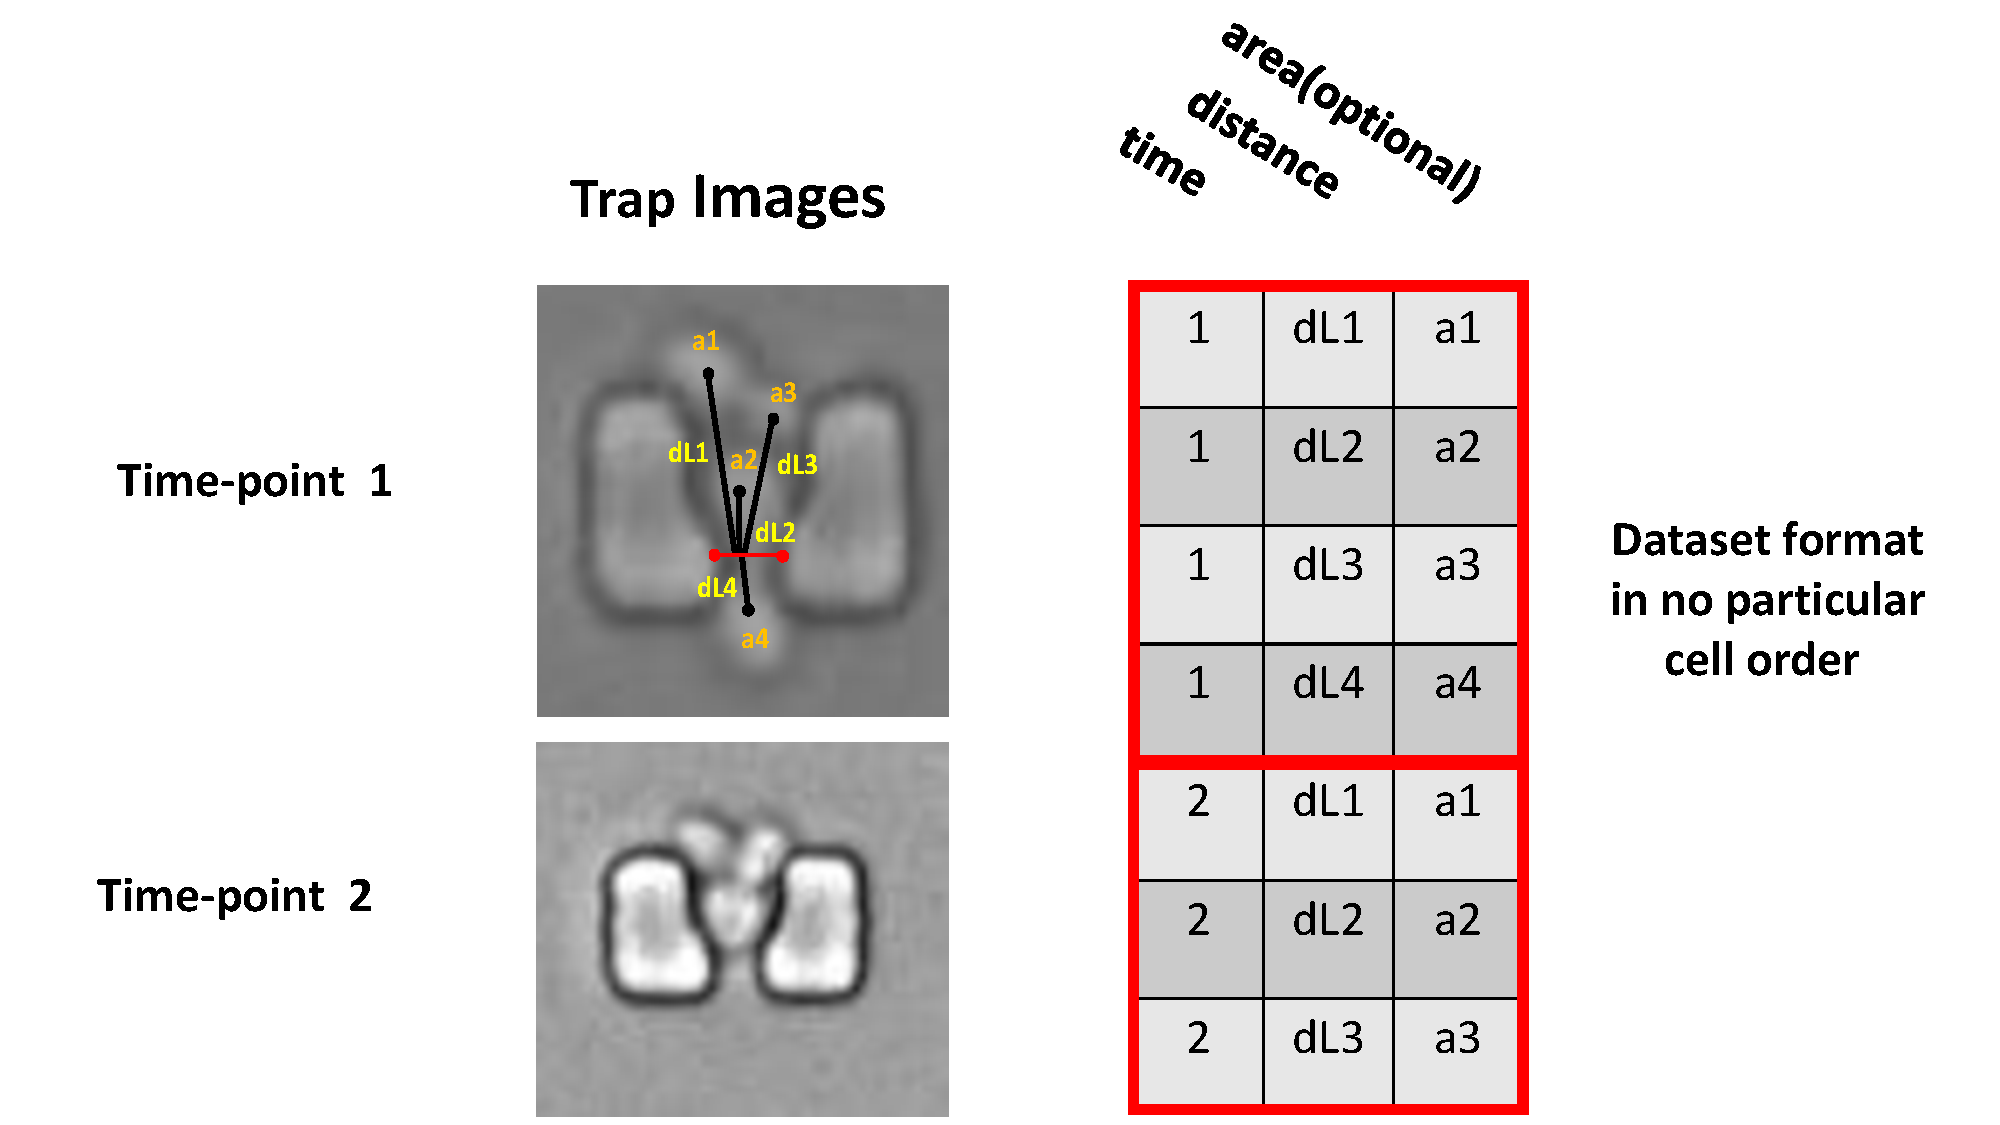
\includegraphics[width=\textwidth,height=10 cm]{Patterns/table.pdf}
\caption{ A sub-image with label for distance and area at time-point 1. A sample table of $\mu$Polar data format at two time-points.}
\label{fig:table}
\end{figure*}


\subsection{$\mu$Polar for microfluidics images}


% Add more details  ................................................

Cell area and offset features could be used for better plot analysis. The cell area could be set to "NA" if the cell area information is not available. Furthermore, the offset value is to adjust the gap between the maximum radius of the dataset and plot out layer. This option could initially set to "NA" and change later on to improve visualization. Fig.\ref{fig:areaoff}(a1) shows a $\mu$polar plot with cell area and offset are equaled to "NA". Fig.\ref{fig:areaoff}(a2) shows $\mu$polar plot with offset value set to 8 where the gap between the maximum radius and plot out layer increase by 8 units. Fig.\ref{fig:areaoff}(b1, b2) show $\mu$polar plot with cell area size decreased and increased by 2 and 8 units respectively. These options are useful for controlling over-size cells and monitoring cell dynamic shape, in particular, if there is no division and cell reached its senescent or over-crowded cells stage.    

\begin{figure*}
\centering
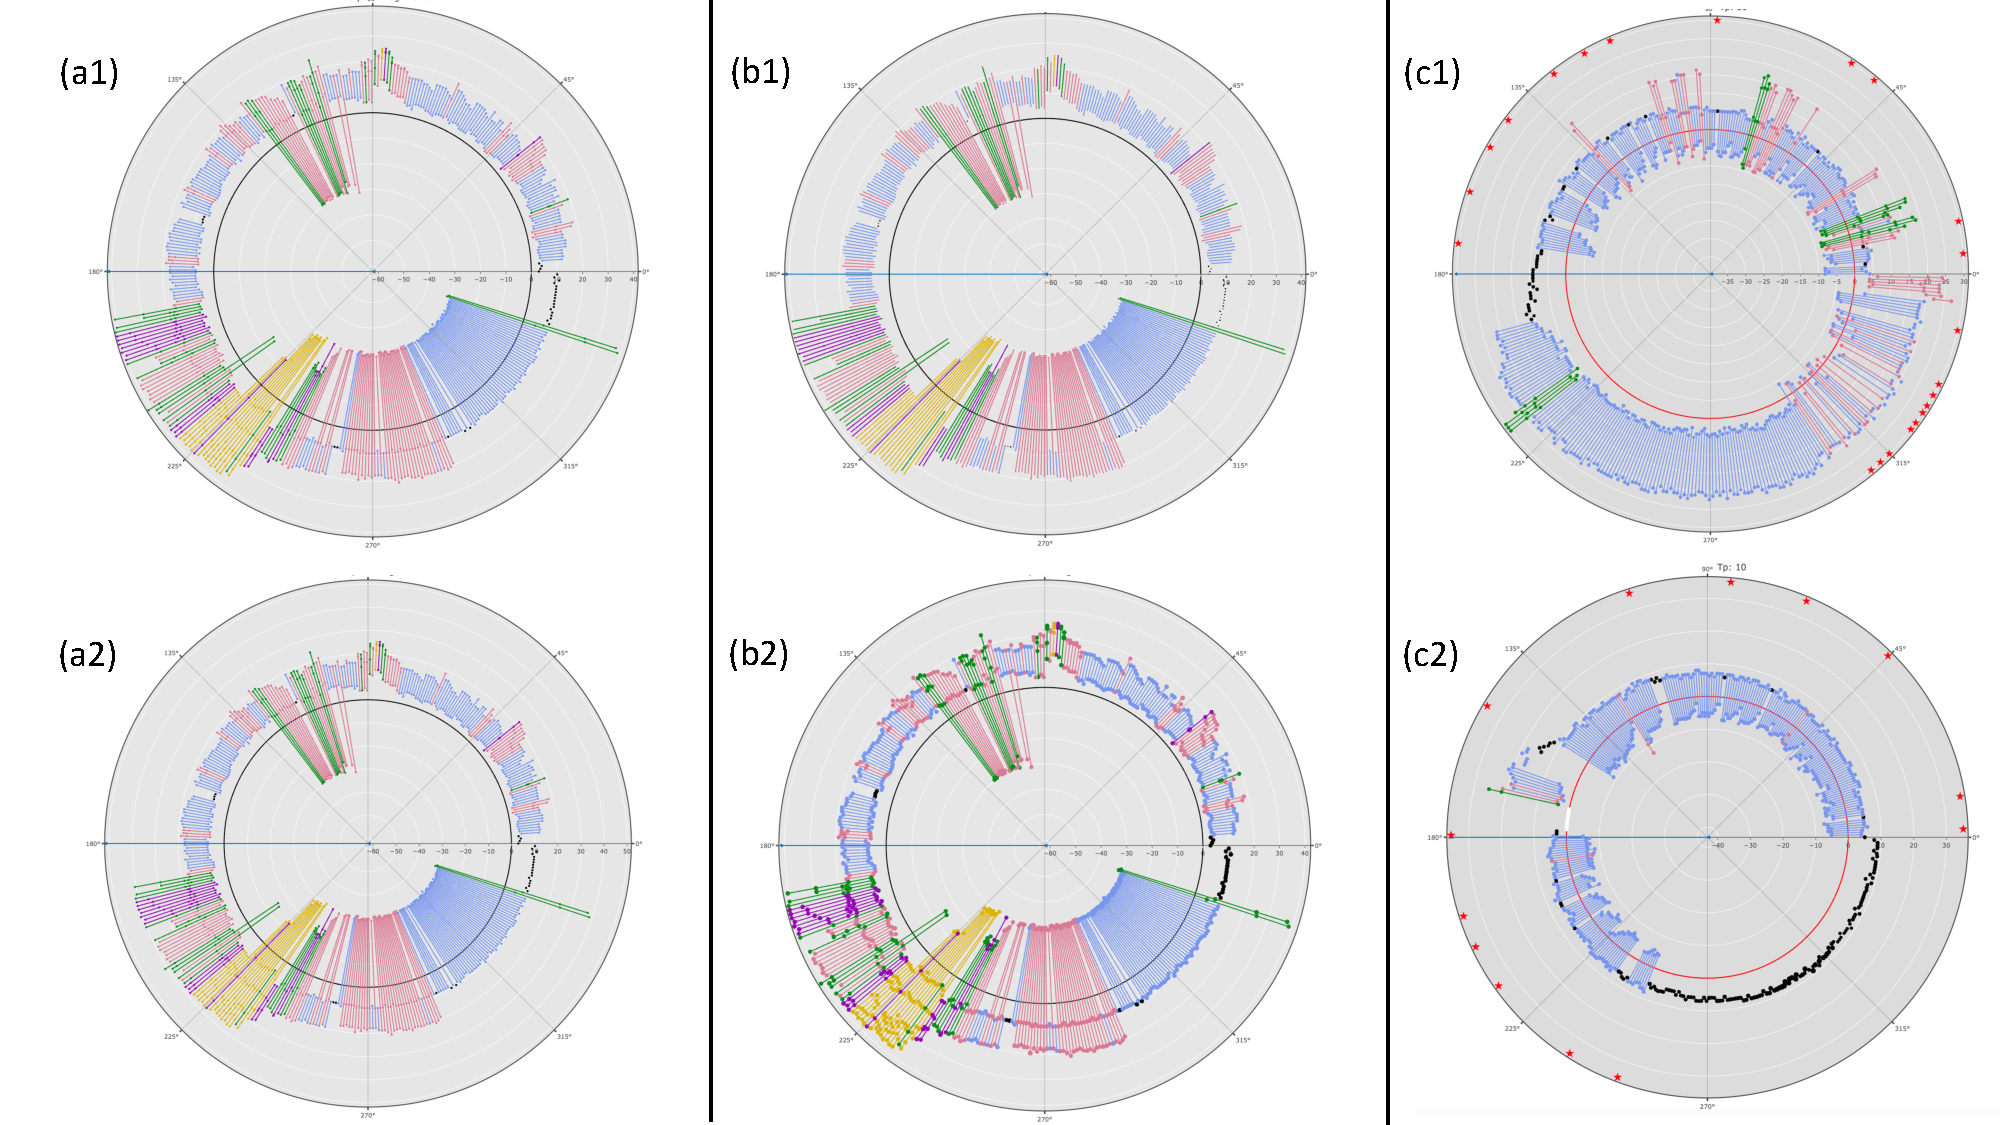
\includegraphics[width=\textwidth,height=10 cm]{Patterns/area_offset.pdf}
\caption{ Example of $\mu$Polar for offset and area features. (a1) and (a2) are related to offset feature example adjusting the cap between cells and plot out layer. (b1) and (b2) are related to area feature example with can be adjustable for better visualization.}
\label{fig:areaoff}
\end{figure*}

\subsection{$\mu$Polar for microscopic images}
In addition to the microfluidics images, we also investigated the $\mu$Polar plot result in the microscopic image. We collected 37 time-lapse microscopic images (dimension = 307x306) from \cite{ref05} as shown in Fig.\ref{fig:scopic}(a). The number of available cells in each image is in range of 50 - 70. For simplicity of plotting, a section of these images cropped in dimension of 121x121 based on average cells availability in a region of interest. (Fig.\ref{fig:scopic}(b)). Correspondingly, feature extraction applied to these images collecting cells coordinate of each image in order of time. According to observation, the cells gradually tend to move to the left direction of images over the time. Thus, the reference point selected at the left-side of images edge (2,150) calculating cell distance. Fig.\ref{fig:scopic}(c) illustrates the $\mu$Polar plot where the cells number are in the range of 6 - 12 indicating different color code. Since the number of cells is 37, the color indication shows a great visualization of cell movement variation. This is very useful for cell monitoring, counting RLS and cell tracking. For instance, the comparison between the closest cell to the center-point at time-point 1 and closest cell to center-point at time-point 37 shows that the amount of cell movement from time-point 1 to time-point 37 is approximately 20 units.        

\begin{figure*}
\centering
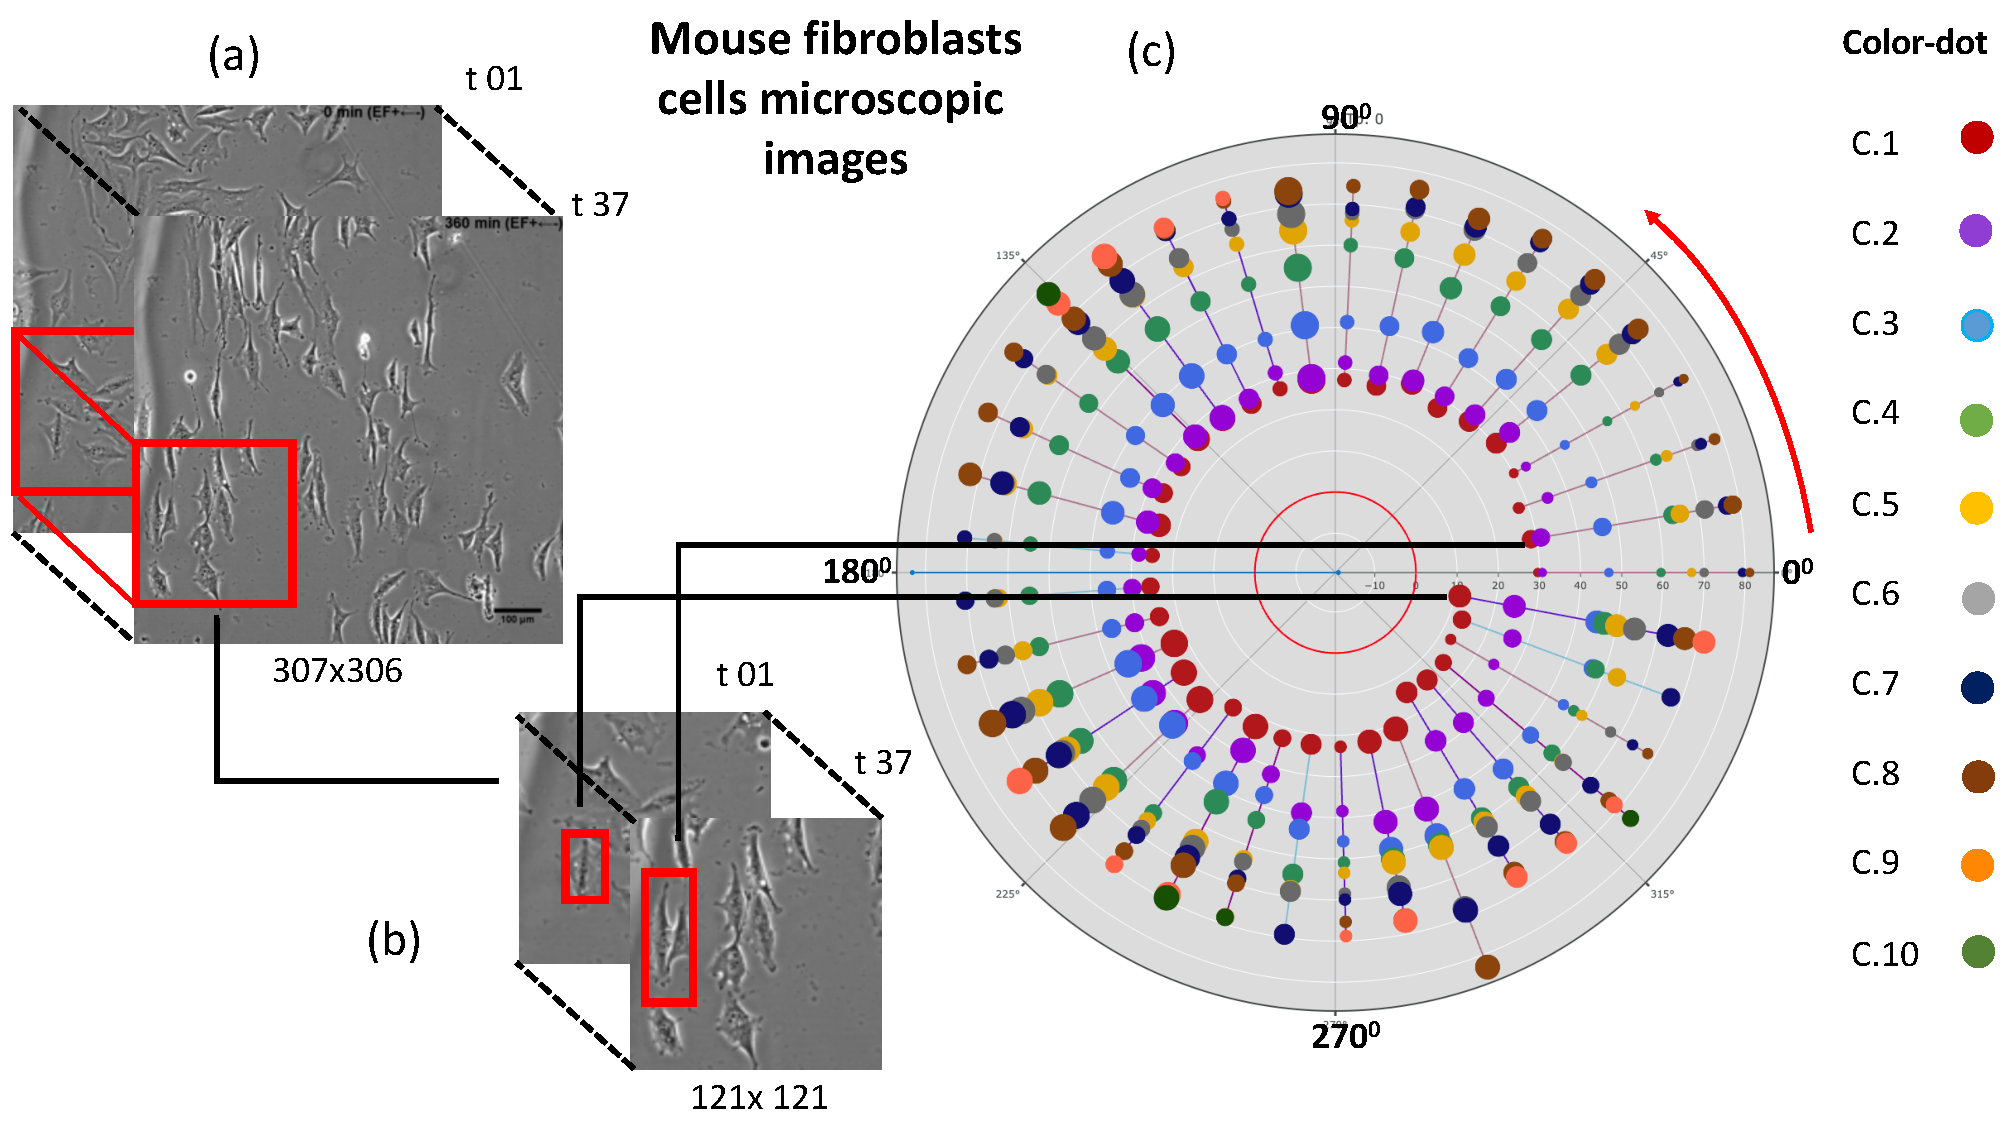
\includegraphics[width=\textwidth,height=10 cm]{Patterns/microscopic.pdf}
\caption{ An example of time-lapse microscopic images applying  $\mu$Polar.}
\label{fig:scopic}
\end{figure*}


\section{Discussion}

Fig.\ref{fig:read} is an overview of some prevalently events from yeast cells time-lapse microfluidics images. Each of the sub-figures is a representation of most common events during the experimental work which can be visualized by $\mu$Polar. The event (a) is representing traps without any present cells which commonly occurs for traps close to the bottom of microfluidics device due to shorten cell life-cycle. The event (b) portends the upcoming division event from potentially mC located inside the trap with a bud at trap outlet. This estimation is based on distance visualization between two cells (mc and bud). In the next event (c), the black dots representing single-cell separation cycle  occurred after bud increased in size the single-cell remains inside the trap. The event (d) shows a single cell inside the trap growing in size. This is most common at the end of the cell lifespan. The (e) and (f) events are good visualization examples of cell division at the absence of a single cell which arguably notifies the occurrence of cell division. In the (e) event, the arrow on the Up region indicates that single-cell inside the trap (black dot) started division and there is not much cell development in size. However, the two arrows indicate that there is a cell attached to the cell inside the trap and its size growing gradually until complete the division cycle, we called this "dC below mC" situation. The (f) event illustrates similar development in the opposite direction when a single call is in steady position and cell above it is growing gradually, we also called this "dC above mC" situation. The (g) demonstrates an event there two cells have been close to each other for sometimes without much development. we realized that this situation occurs when cells becoming older and interestingly the cell separation cycle becoming longer. $\mu$Polar could potentially be a great Visualization tool to compare a cell separation cycle time at its early lifespan and cell separation cycle time at its late lifespan. The (h) shows overcrowded events when the number of cells in the image reaches more than two cells where each color representing a different number of cells.

\begin{figure*}
\centering
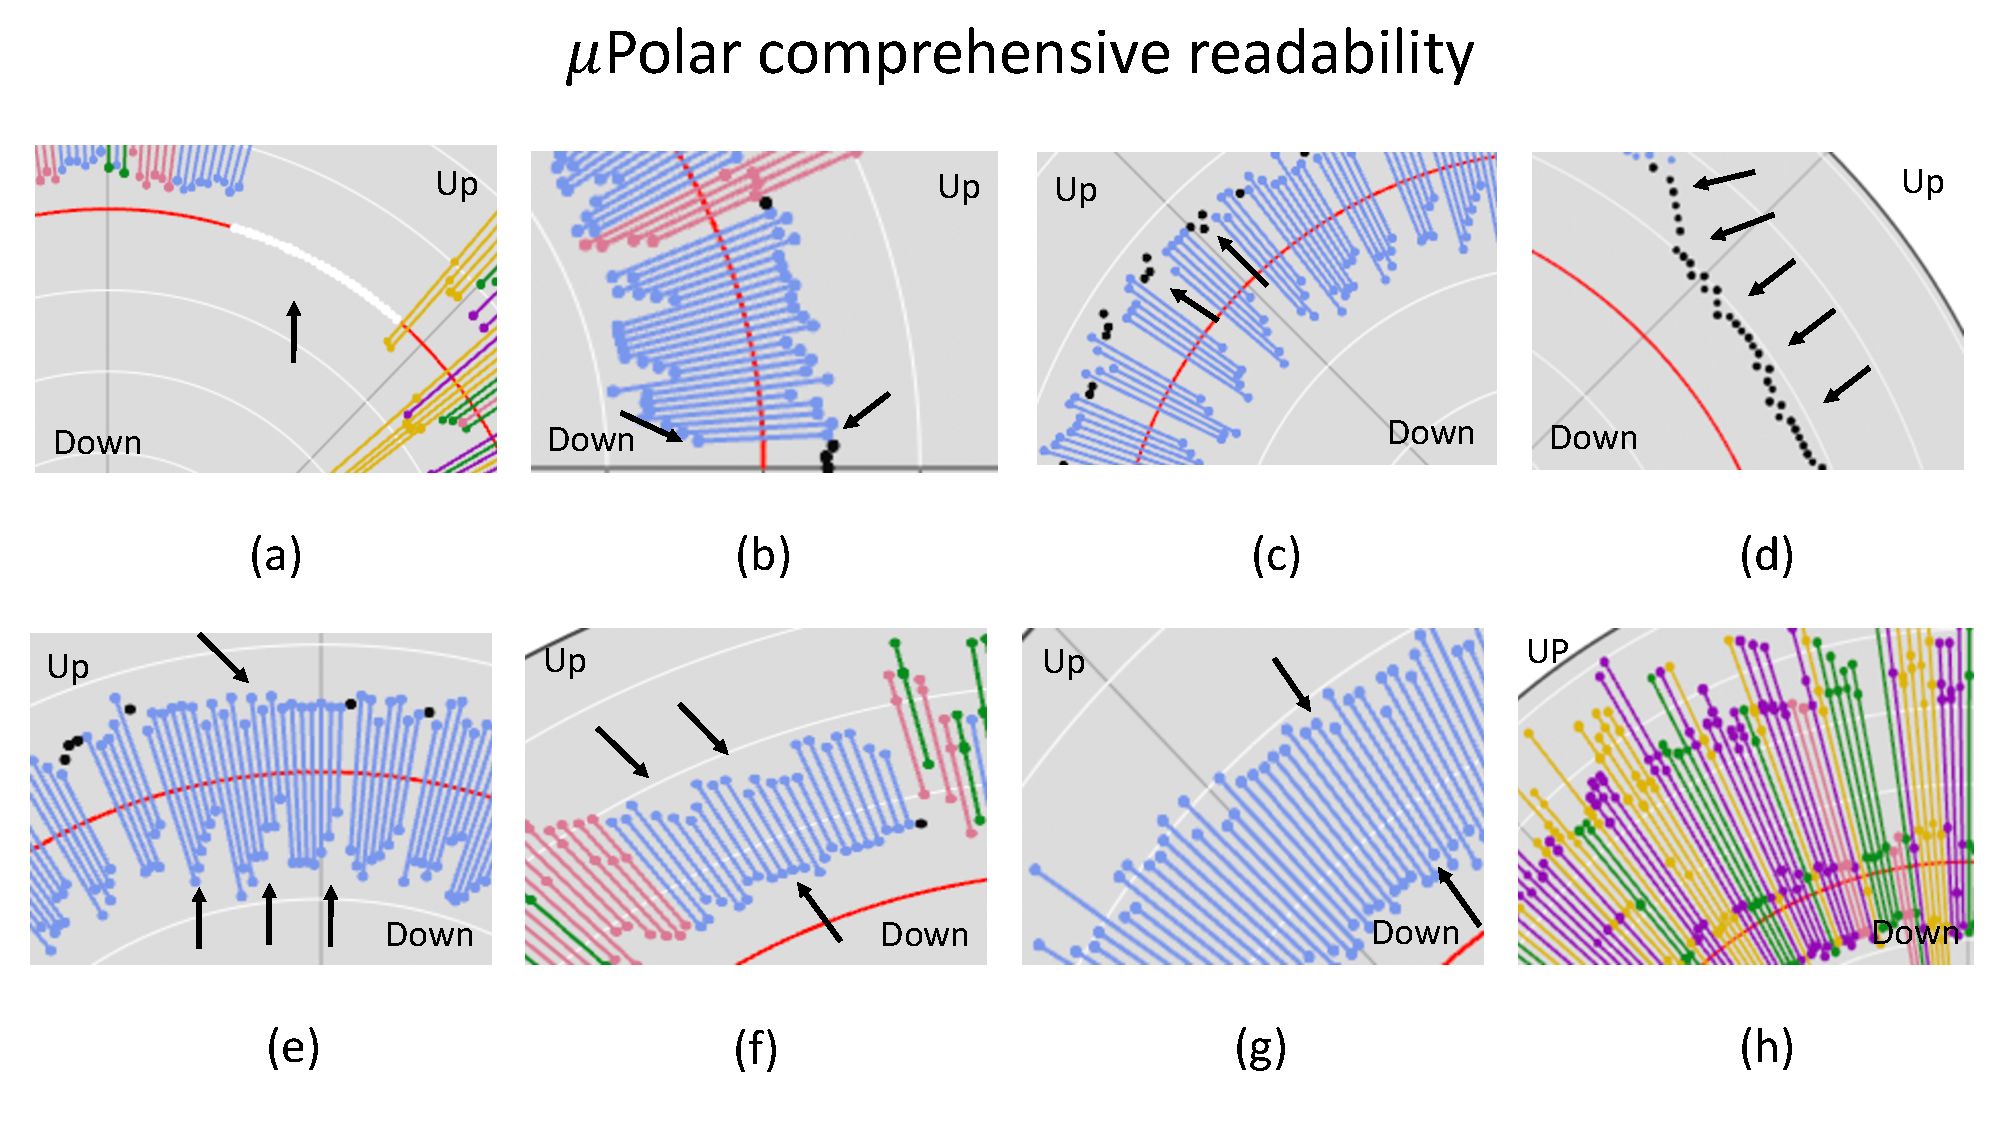
\includegraphics[width=\textwidth,height=10 cm]{Patterns/read.pdf}
\caption{Readability of some common cellular events for yeast cells. Any event occurred below the reference line (passed trap outlet) denoted as "Down" and any events occurred above the reference line (inside and above trap) denoted as "Up". (a) The white dots (pointed with arrow) on the red reference line are indications of the trap without cell. (b) The two arrows pointing each other are indicating that a single cell (black dot) started a division, cells are at an early age and very close to each other (one inside the trap, one outside trap outlet). (c) The Black dots are representing a division after two cells completed the separation cycle. (d) The representation of a single cell inside trap growing size over time. (e) The arrow on the Up region indicates that there a cell inside trap without much growing in size. That arrows on down region indicate that there is a single cell below and close to the cell inside the trap and gradually growing in size until complete separation which we called this even "dC below mC". (f) The arrow on down region indicates that there is a single cell inside trap without much growing in size. The two arrows are indicating that there is a cell above and close to the cell inside the trap and growing in size until complete separation which we called this event "dC above mC". (g) The arrows show two cells attached inside the trap and have not completed the separation cycle for sometimes. (h) Indication of the events of the overcrowded cell occurred sometimes.(h) Indication of the over crowded cells events occurred for sometimes.}

\label{fig:read}
\end{figure*}

Fig.\ref{fig:explain} demonstrates an overview of a single trap for the cells division process over time. In this $\mu$Polar plot, cells are shown in five colors, black color represents single mother cell(mC), light blue represents two cells, pink color represents three cells, green color represents four cells and purple color represents five cells. We considered this plot with six stages over time-point 1 to time-point 391. At stage one (0 - 170 degree), the light blue color representing traps with presents of two cells where the mother cell (mC) is located inside the trap and the daughter cell (dC) passed reference line (red line) located at trap outlet. At stage two (170 - 190 degree), the mC remains inside the trap and the dC located above mC.  An example of these stages is illustrated in Fig.\ref{fig:explain}. At stage three (190 - 260 degree), multiple colors representation show that there is an over-crowded situation inside and above the trap. AT stage five ( 260 - 350 degree), there are constantly two cells available inside the trap and there is no sign of division or development. Potentially, this is the cell senescence stage and follows by cell dead stage. The comparison of stage one and stage two shows that the distance between two cells is increased, no single cell passed trap outlet and cell size is bigger representing old cells    


\begin{figure*}
\centering
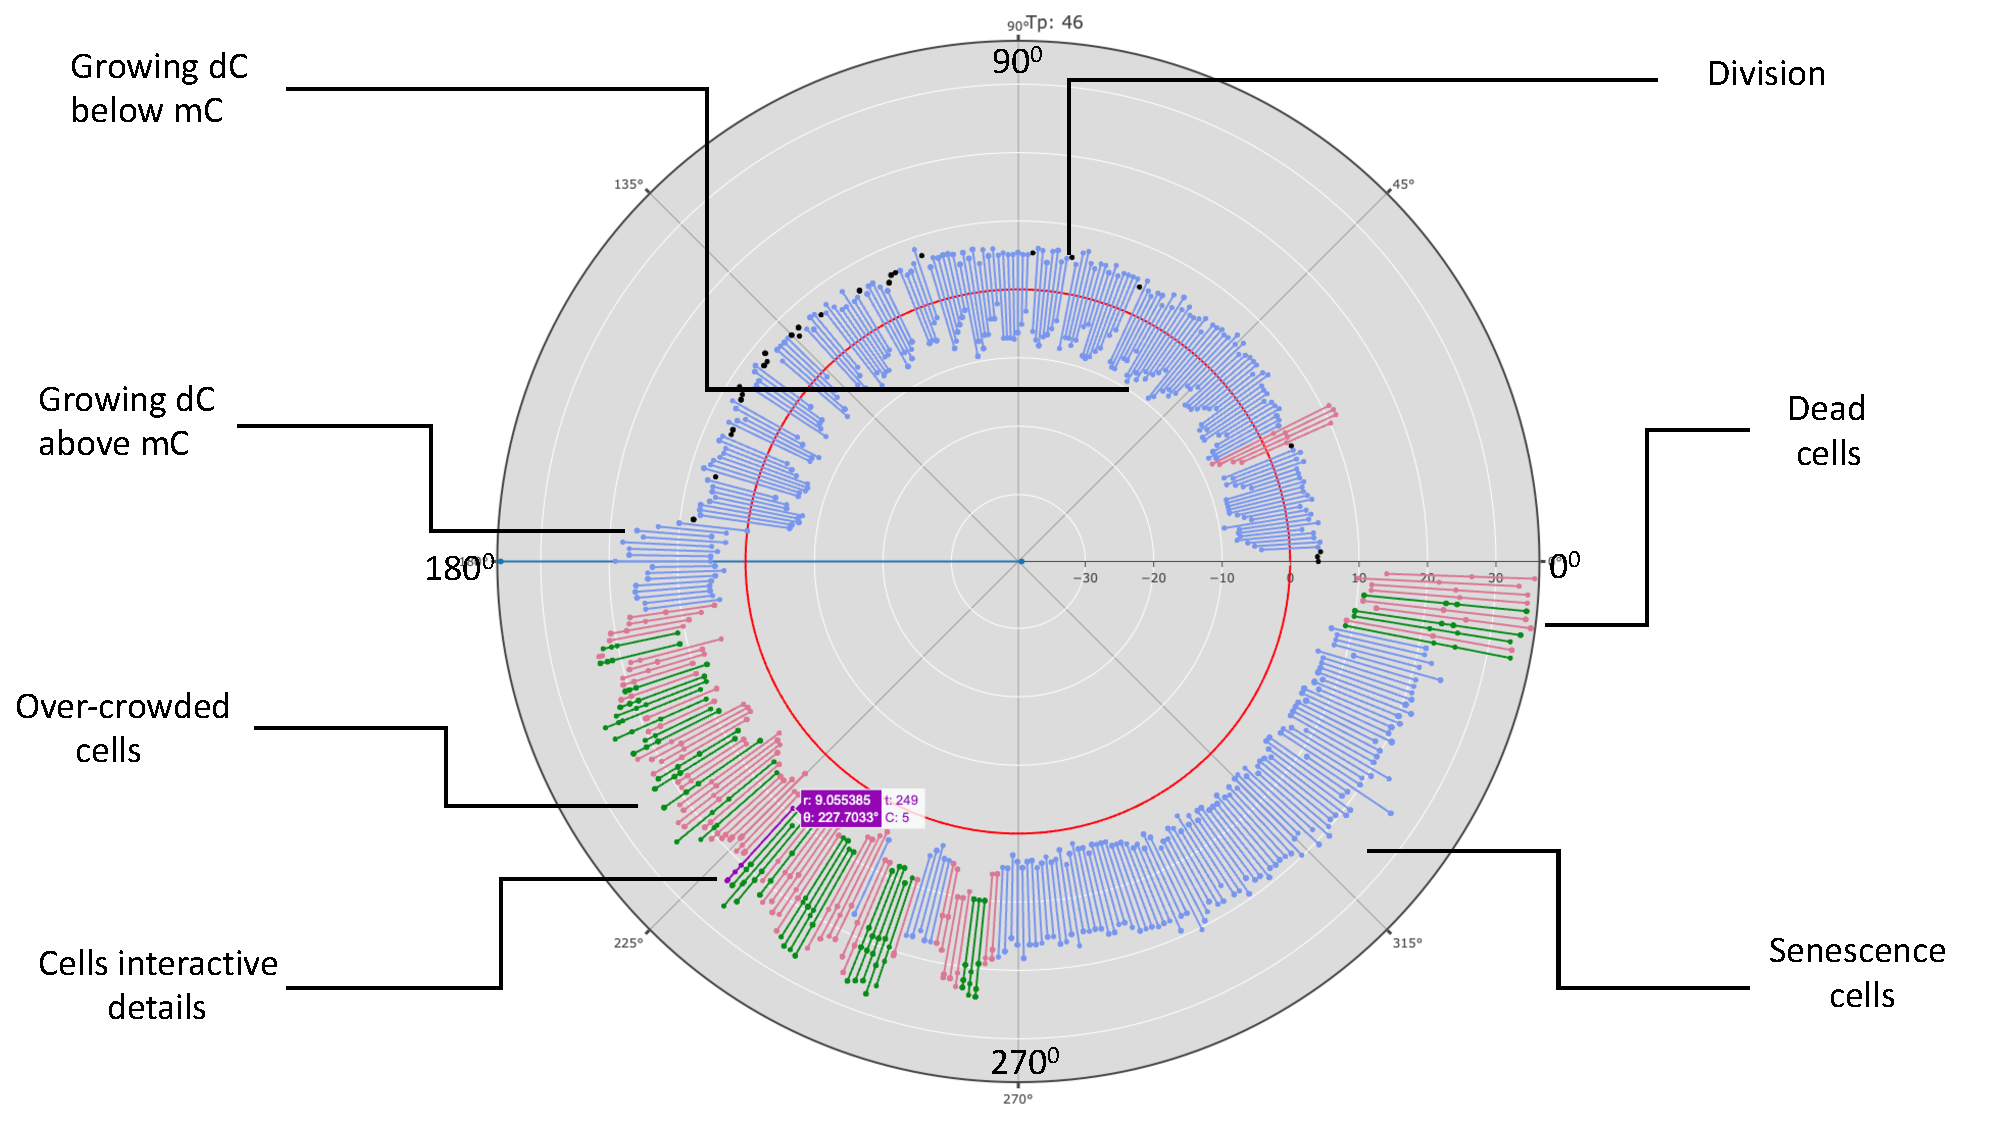
\includegraphics[width=\textwidth,height=10 cm]{Patterns/explain.pdf}
\caption{A trap example analysis with $\mu$Polar plot for time-points 1 - 391.}
\label{fig:explain}
\end{figure*}


\subsection{$\mu$Polar RLS}

$\mu$Polar has an additional option for replicative lifespan (RLS) visualization. This feature could be added to the plot if RLS dataset is available from the dataset. The RLS division points appear inside the plot out layer with a "star" sign. Fig.\ref{fig:rls} demonstrates the comparison of two $\mu$Polar plots from the same trap with different RLS counting methods. We previously collected the trap RLS data from \cite{ref02.2} and applied this information to the $\mu$polar. Fig.\ref{fig:rls}(a) shows $\mu$polar plot with countable red color "star" representing trap RLS from collected data. In this particular example, there are 13 red "stars" corresponding to the trap RLS. Fig.\ref{fig:rls}(b) shows $\mu$Polar plot for same the trap without collected RLS dataset. In this example, we counted the potential division and labeled time-points denoted with "Triangle". There are 13 "triangles" corresponding to the trap RLS. This example is based on good scenarios and used for RLS estimation. Therefore, the comparison shows that the prior RLS data could be displayed by $\mu$Polar for visualization purposes and additionally, the RLS could be estimated from $\mu$Polar plot. To have better visualization and avoid overlapping, it is advisable to set offset and c.Adjust values properly.       

\begin{figure*}
\centering
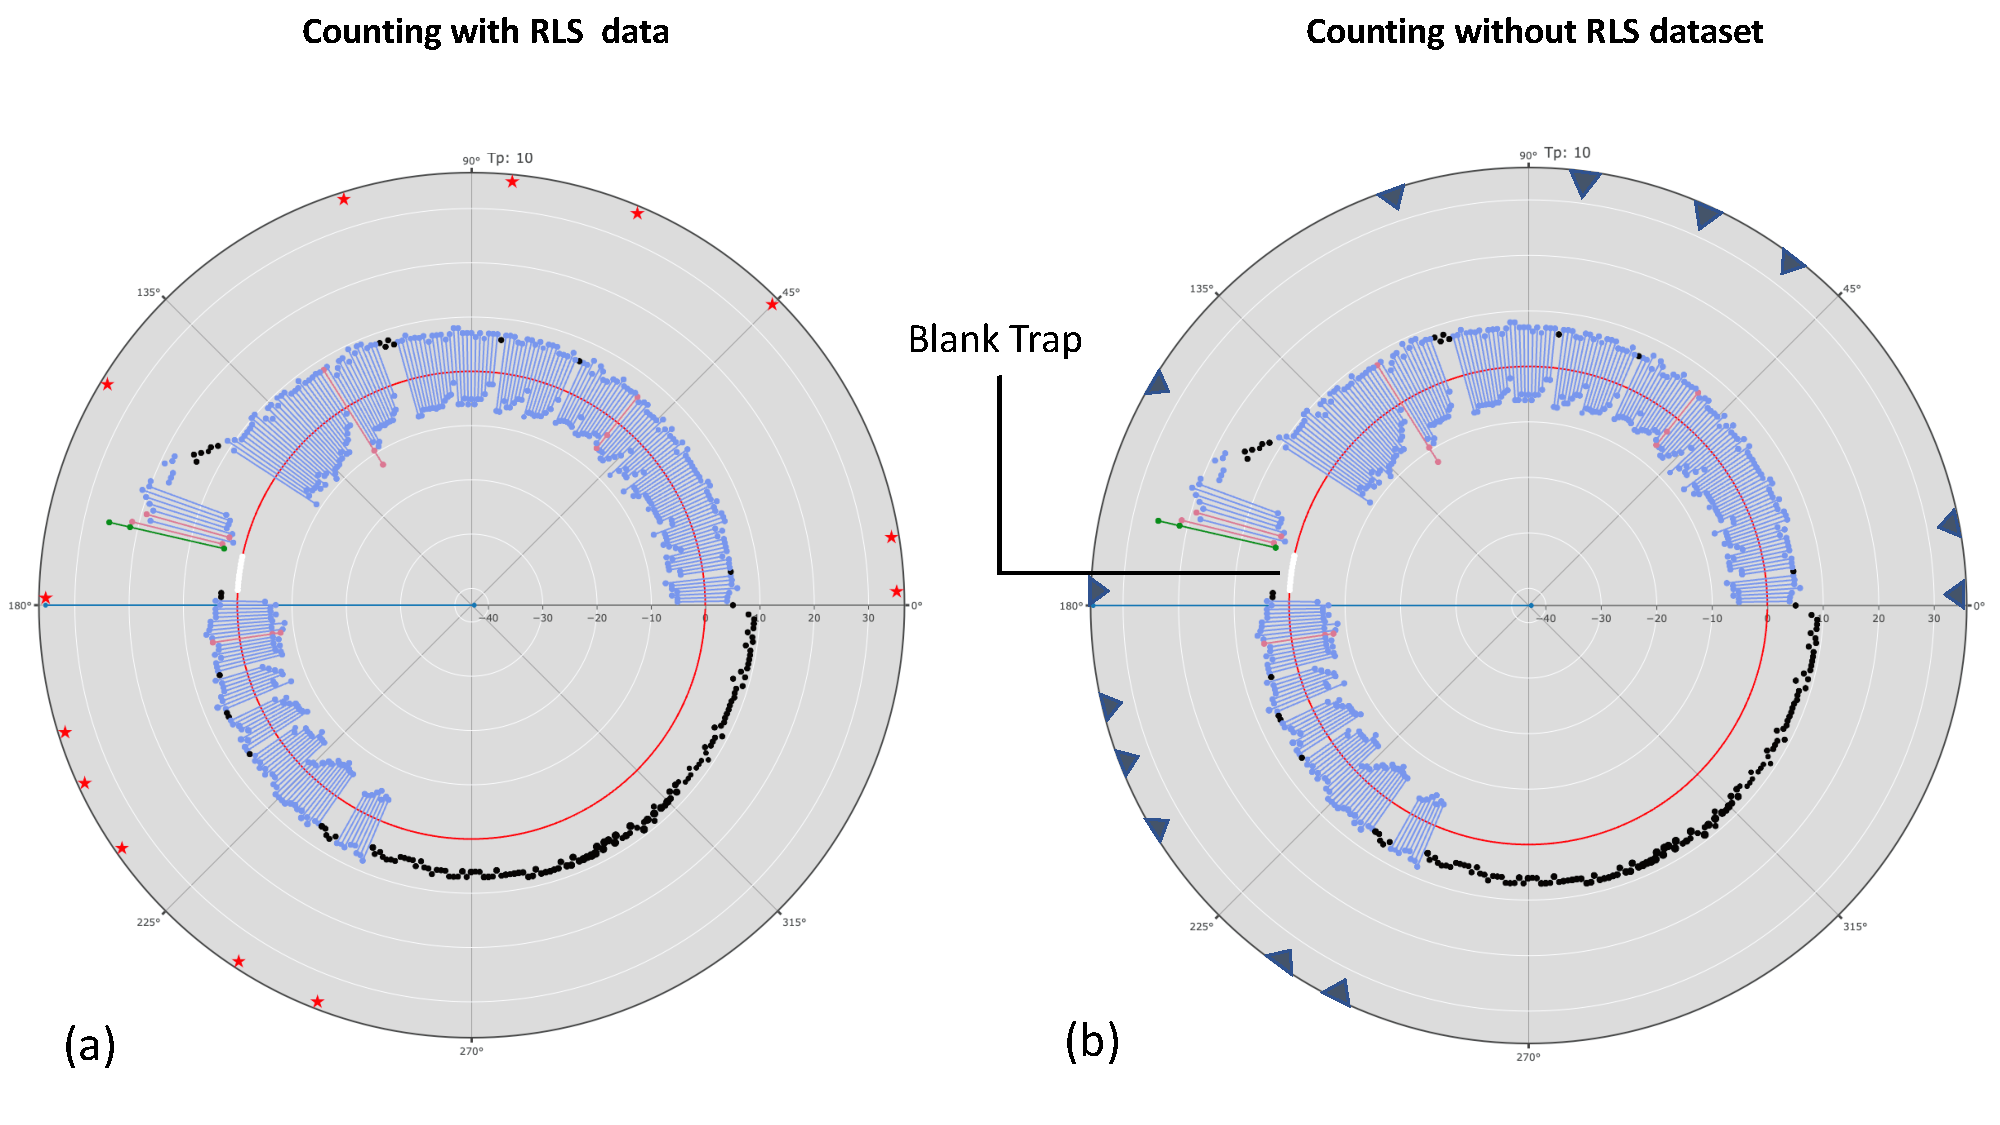
\includegraphics[width=\textwidth,height=10 cm]{Patterns/rls10.pdf}
\caption{ Identify the number of RLS from $\mu$Polar without RLS dataset. (a) A $\mu$Polar plot from a trap with prior RLS counting dataset represented by "stars". (b) A $\mu$Polar plot for same trap without collected RLS dataset represented by "triangle" counted from plot division points.}
\label{fig:rls}
\end{figure*}

Fig.\ref{fig:division} represents a situation that could lead to RLS miscounting during a  experimental work. This example show a sequence of images from time-point 30 to 59 with corresponding $\mu$Polar plot. The time-point 47 and time-point 48 are representing two cells cell with steady cell inside the trap. The $\mu$Polar shows great visualization of the cell development at trap outlet from time-points 47 - 48 which can justify the occurrence the cell division. The $\mu$Polar visualization analysis can improve cell replicative lifespan accountability for the aging process.    

\begin{figure*}
\centering
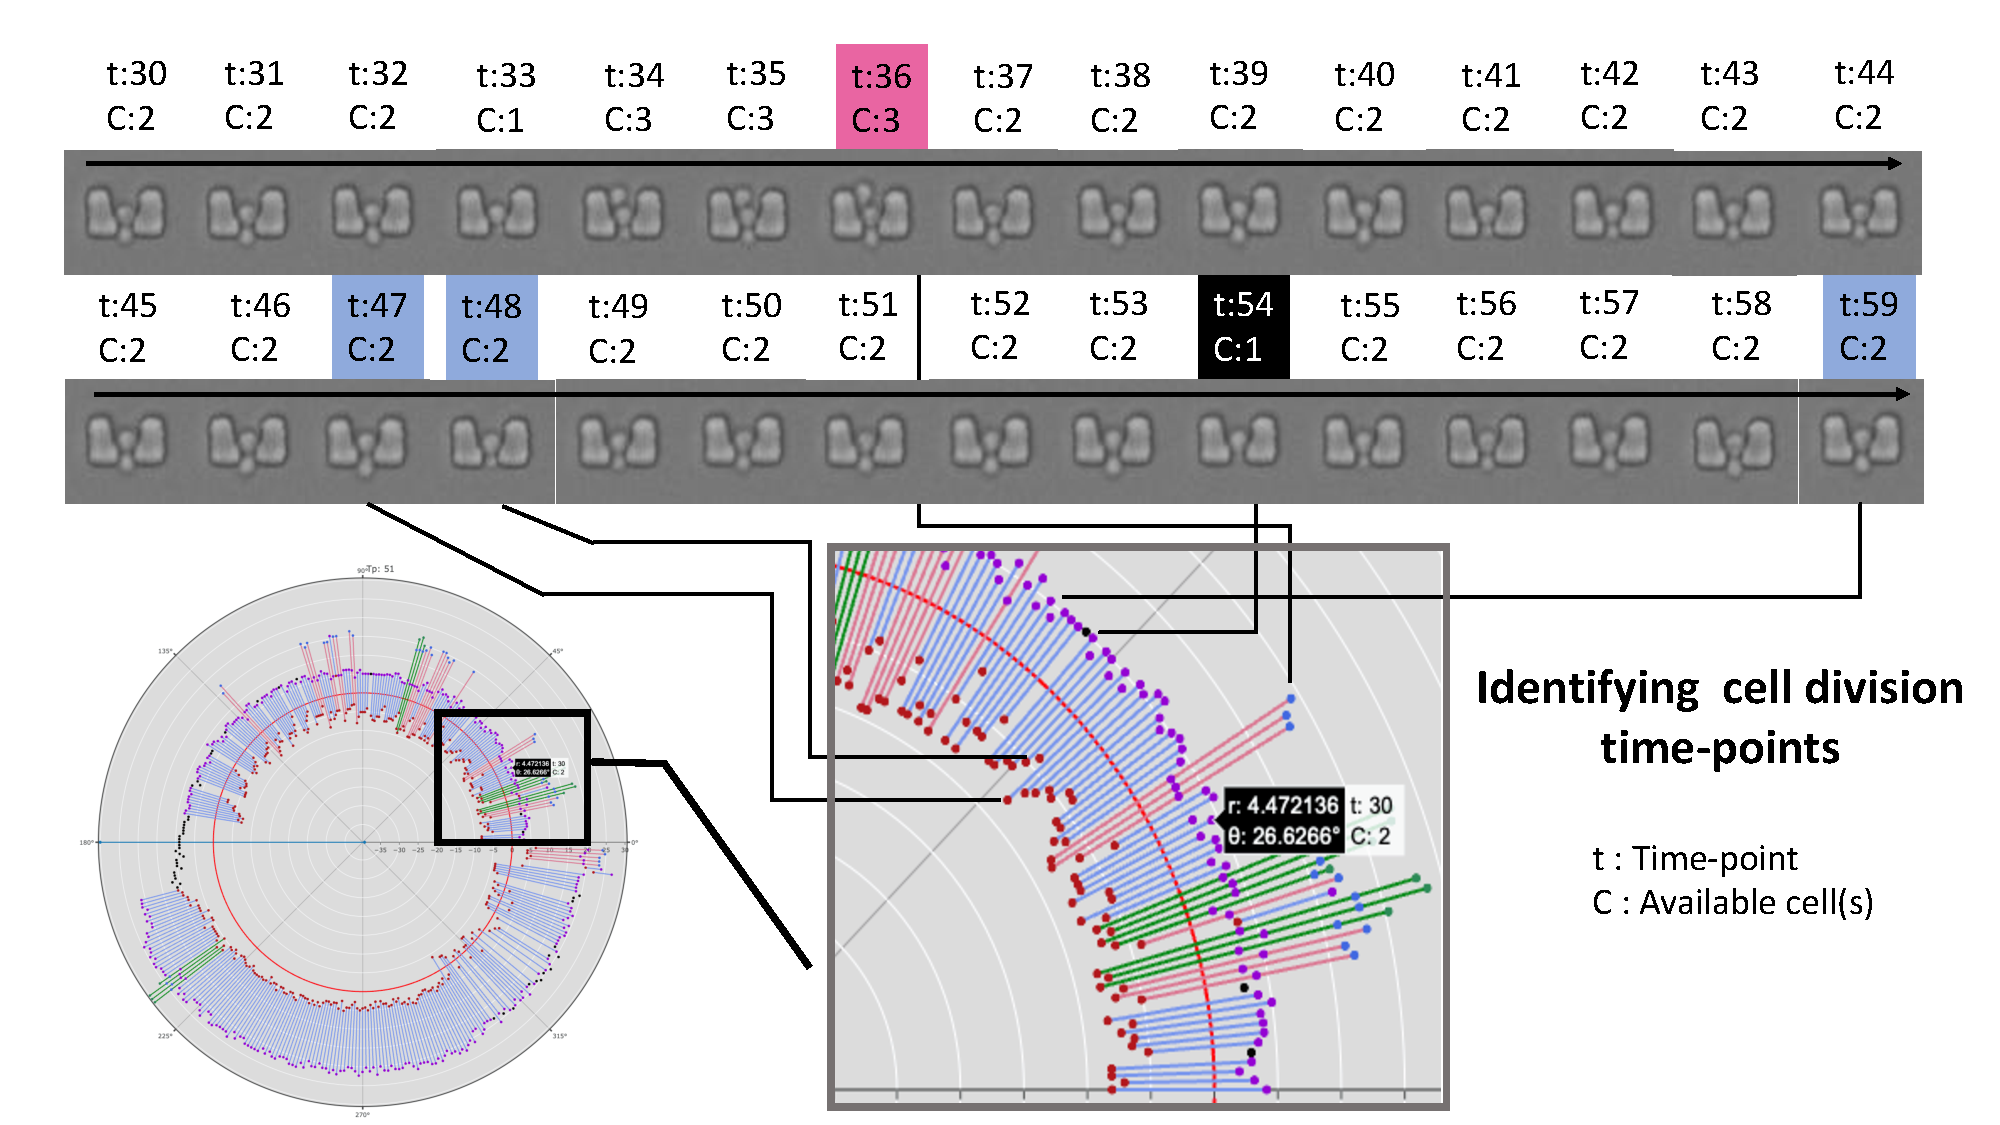
\includegraphics[width=\textwidth,height=10 cm]{Patterns/division.pdf}
\caption{ Representation of microfluidics time-lapse images from time-points 30 to 59 with number of available cell(s). The time-point 35(pink) indicates the number of cells decreasing from three to two. Time-points 47 to 48 indicate the occurrence of cell division. The time-point 53 represents a single cell inside trap (black).}
\label{fig:division}
\end{figure*}


\section{Star*Methods}

\subsection*{Data collection}
The microfluidics sequence images are procured from \cite{ref13} recent experimental work. The high-throughput yeast aging analysis (HYAA) chips device is a composed Polydimethylsiloxane (PDMS) model that contains 16 individual channels combined into four modules as shown in Fig.\ref{fig:micro}(a).

\begin{figure*}
\centering
\includegraphics[width=\textwidth,height=10 cm]{Patterns/fluidics.pdf}
\caption{ HYAA microfluidics chips. (a) Four modules (16 channels) microfluidic device. (b) A time-point sample of microfludics image shown with guidelines 10 - 70. (c) An example of time-lapse ( t1-t391) images for guidelines 10 - 20. (d) A sample of time-lapse (t1 - t391) partitioned images (60x60).}
\label{fig:micro}
\end{figure*}

All time-lapse microfluidics images are captured with IX-81 Olympus inverted microscope equipped with an Olympus camera (DP72 CCD) operating by cellSens software. The experimental process took around 96 hours at a temperature of 86$^{\circ}$F (30$^{\circ}$C). Each channel has 520 traps inside the microfluidic chamber and each row has 7 or 6 traps consecutively. Channels are labeled with numbers right-side for capturing guidelines. The order of rows could be different depending on capturing adjustment. For instant, if the camera positioned on guidelines 10 and 20, the first row of the captured image starts with 7 traps and so on. The experiment ended with capturing 391 images with 10 minutes interval. Images are captured at four locations of the microfluidic device ( Fig.\ref{fig:micro}(b)). 1st position: camera covered guidelines 10 - 20. 2nd position: camera covered guidelines 30 - 40. 3rd position: camera covered guidelines 50 - 60. 4th position: camera covered guideline 70. In this work, we have considered the dataset from 1st position (10 - 20) as shown in Fig.\ref{fig:micro}(c).

\subsection{Data Pre-processing}
Since microfluidics images have relatively low resolution and are considered a challenging task for visualization, we partitioned every single image to sub-images based on the individual trap. Traps are labeled from time-point 1 to time-point 391 as illustrated in Fig.\ref{fig:micro}. All sub-images partitioned concerning local traps boundary at 60x60 dimension. We used You Only Look Once (YOLOv3) \cite{ref20} machine learning model for image feature extraction. We collected 391 sequence sub-images for each trap, extract and label them as following: "time" (image time number), "distance (cell distance from reference point) and cell "area" (Fig.\ref{fig:table}). The cell features in each image are collected in no particular order (e.g, cell size, location). However, the features of each image are collected in order of time. For instance, Fig.\ref{fig:table} shows that the features of the first image input with four cells are collected indicating four rows for each cell and assigning time number (time) one for all of them. This labeling method continuously followed for the rest of the images.

\subsection{Distance calculation and time-points conversion}
The process of feature extraction carried on for 104 available traps as illustrated in Fig.\ref{fig:micro}(c). We then surcharged individual cell distance feature from the existing dataset by using the euclidean equation:

\begin{equation}
\begin{split}
d_i = \sqrt{(x_i -x_r)^2 + (y_i -y_r)^2}\\
\\
i =  [1,2,3,4,..., m ] \\
\\
\end{split}
\end{equation}

where $ d_i $ is the distance between the centroid point of cell and reference point. $ x_i $ and $ y_i $ are cells coordinate at each image. $ x_r $ and $ y_r $ are trap reference point. Generally, these points could be chosen at any point of image based on region of interest. We decided to choose the reference point based on cell flow direction and potential cell division point. $ i $ is image number corresponding to time-point and $ m $ is the maximum time-point equivalents to total number images. Here, $ x_r $ and  $ y_r $ are set to be 30 and 34 respectively at trap outlet as shown in $\nameref{S1_Fig}$. In a further step, we converted time to degree by using: 
 
\begin{equation}
\begin{split}
 degree = \sum_{i=1}^{n}{theta_i}\\
 \\
\end{split}
\end{equation}

here, $theta $ = \text{maximum degree}$/$\text{maximum time} and $ degree $ is accumulative degree of each radius and $ n $ is equal to maximum degree (e.g, 360). All distance values are considered as radius for cell movement interpretation.     


\subsection{$\mu$Polar input}

Fig.\ref{fig:table} illustrates an example of traps at time-points 1 and 2. Time-point 1 shows the label for distance and area of each cell. dL1, dl2, dL3, and dL4 are a distance from reference point. a1, a2, a3 and a4 are area of each cell. The table in Fig.\ref{fig:table} represents an example of the $\mu$Polar dataset format at two time-points. The dataset feature is labeled as following; "time" (image time number), "distance" (cell distance to reference point) and "area" (cell area)  which is optional and can be used for cell size variation visualization. Image at time-point 1 belongs to rows 1 - 4 of table dedicating image with four cells and image at time-point 2 belongs to row 5 - 7 dedicating image with three cells.



\subsection{$\mu$Polar visualization paradigm}

Fig.\ref{fig:polar}(a) is an interpretation of a trap sequence images from time-point 1 to time-point 391. The color representation is based on the number of available cell(s) in an image. Here, we used default setting where white color represents trap without cell, black color represents trap with one cell, green color represents trap with two cells, light-brown represents trap with 3 cells, blue color represents trap with 4 cells, orange color represents trap with 5 cells and sky-blue color represents trap with more than 5 cells. Furthermore, the red circle color represents trap reference line. For instance, time-point 275 to time-point 313 and time-point 353 to time-point 360 are represented in white color and laid on reference line (red). $ t  $ and  $ Ce $  are image time-point number and number of available cell(s) respectively. An example of $\mu$Polar plot given at time-point 21 where cell color shown in black since there only single-cell available. 

Fig.\ref{fig:polar}(b) shows a schematic of $\mu$Polar with some sample time-points from a trap. Images at time-points 1 - 6 are represented in $\mu$Polar plot. The theta for time-points 1 - 6 are 0 ,0.92, 1.84, 2.76, 3.68, 4.6 respectively. The plot has two regions separated with red circle, denoted as $ A $ region (cell above reference line) and $ B $ region (cell below reference). In this example, "White" color represents traps without cell located on reference line based on image theta, "black" color represents traps with single-cell located on radius line based on cell distance and image theta, "green" color represents traps with two cells located on radius line based on cell distance and image theta and "orange" color represents traps with three cells located on radius line based on cell distance and image theta. The cell size variation is based on the cell area. The number of cell(s) on each time-point radius indicates the number of cell (s) on each image. For instance, there is no cell at time-point 1, there are two cells at time-point 2, three cells at time-point 3, three cells at time-point 4, two cells at time-point 5 and one cell at time-point 6 respectively


\begin{figure*}
\centering
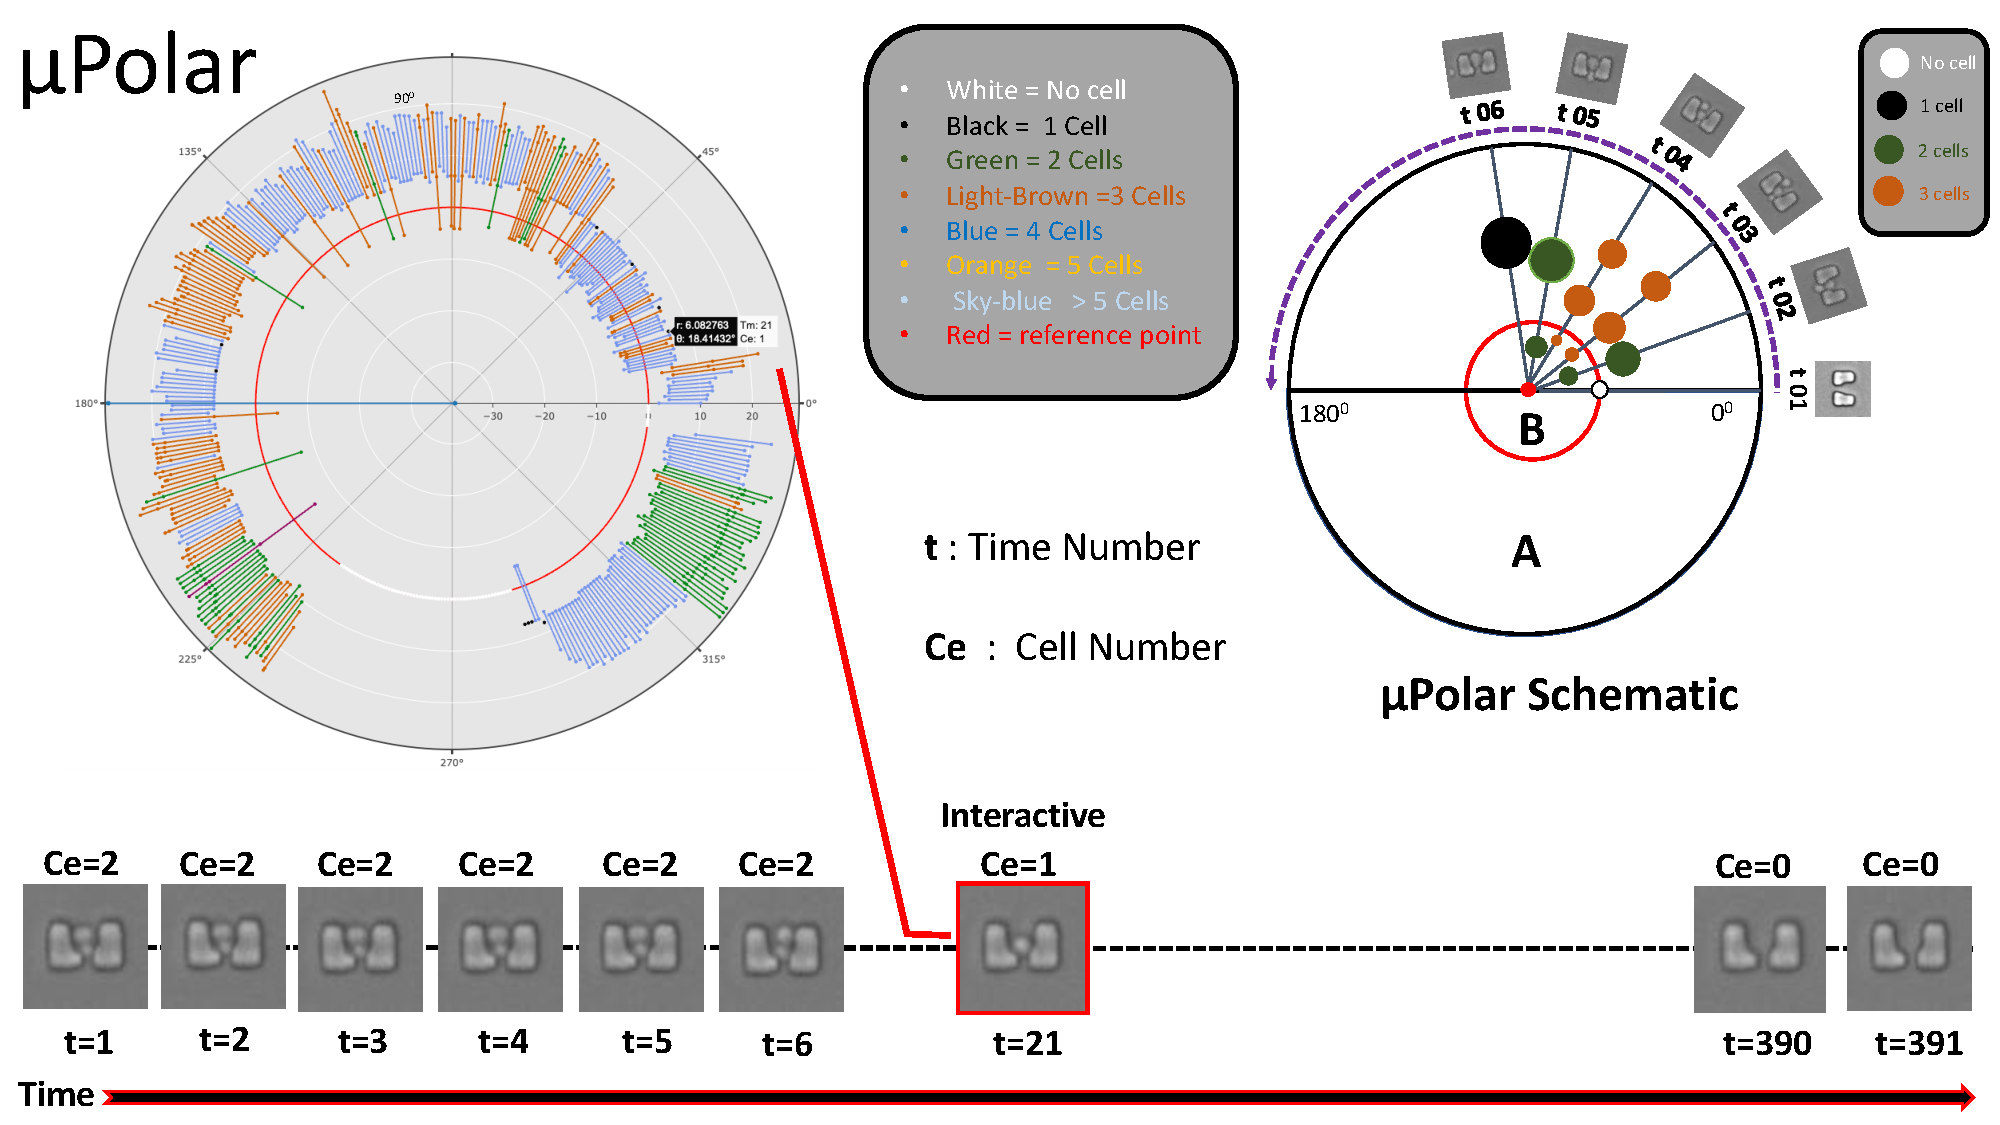
\includegraphics[width=\textwidth,height=10 cm]{Patterns/polar.pdf}
\caption{A schematic and plot examples of $\mu$Polar. (a) $\mu$Polar plot representation of microfludics time-lapse images from time-points 1 - 391. (b) $\mu$Polar schematic representation for time-lapse images from time-points 1 - 6 with indication of number of cell(s) with color codes.}
\label{fig:polar}
\end{figure*}


\section{Conclusion}
Microfluidics-based microscopy is becoming an increasingly popular research tool to monitor cellular events in biomedical research. One such application is the high-throughput analysis of dividing yeast cells. It is challenging to visualize and interpret the data gathered through microfluidics-based microscopy. Here, we developed a circular plotting method, $\mu$Polar, to visualize cell movements and cellular division events at hundreds of time points. Our method is interactive and easy to use. We demonstrated the utility of our method to describe the events of dividing yeast cells. Our method could be potentially applied to other types of microfluidic devices.
This software is implemented in an R package $\mu$Po available through GitHub from https://github.com/merang/uPolar.


% \begin{figure*}
% \centering
% 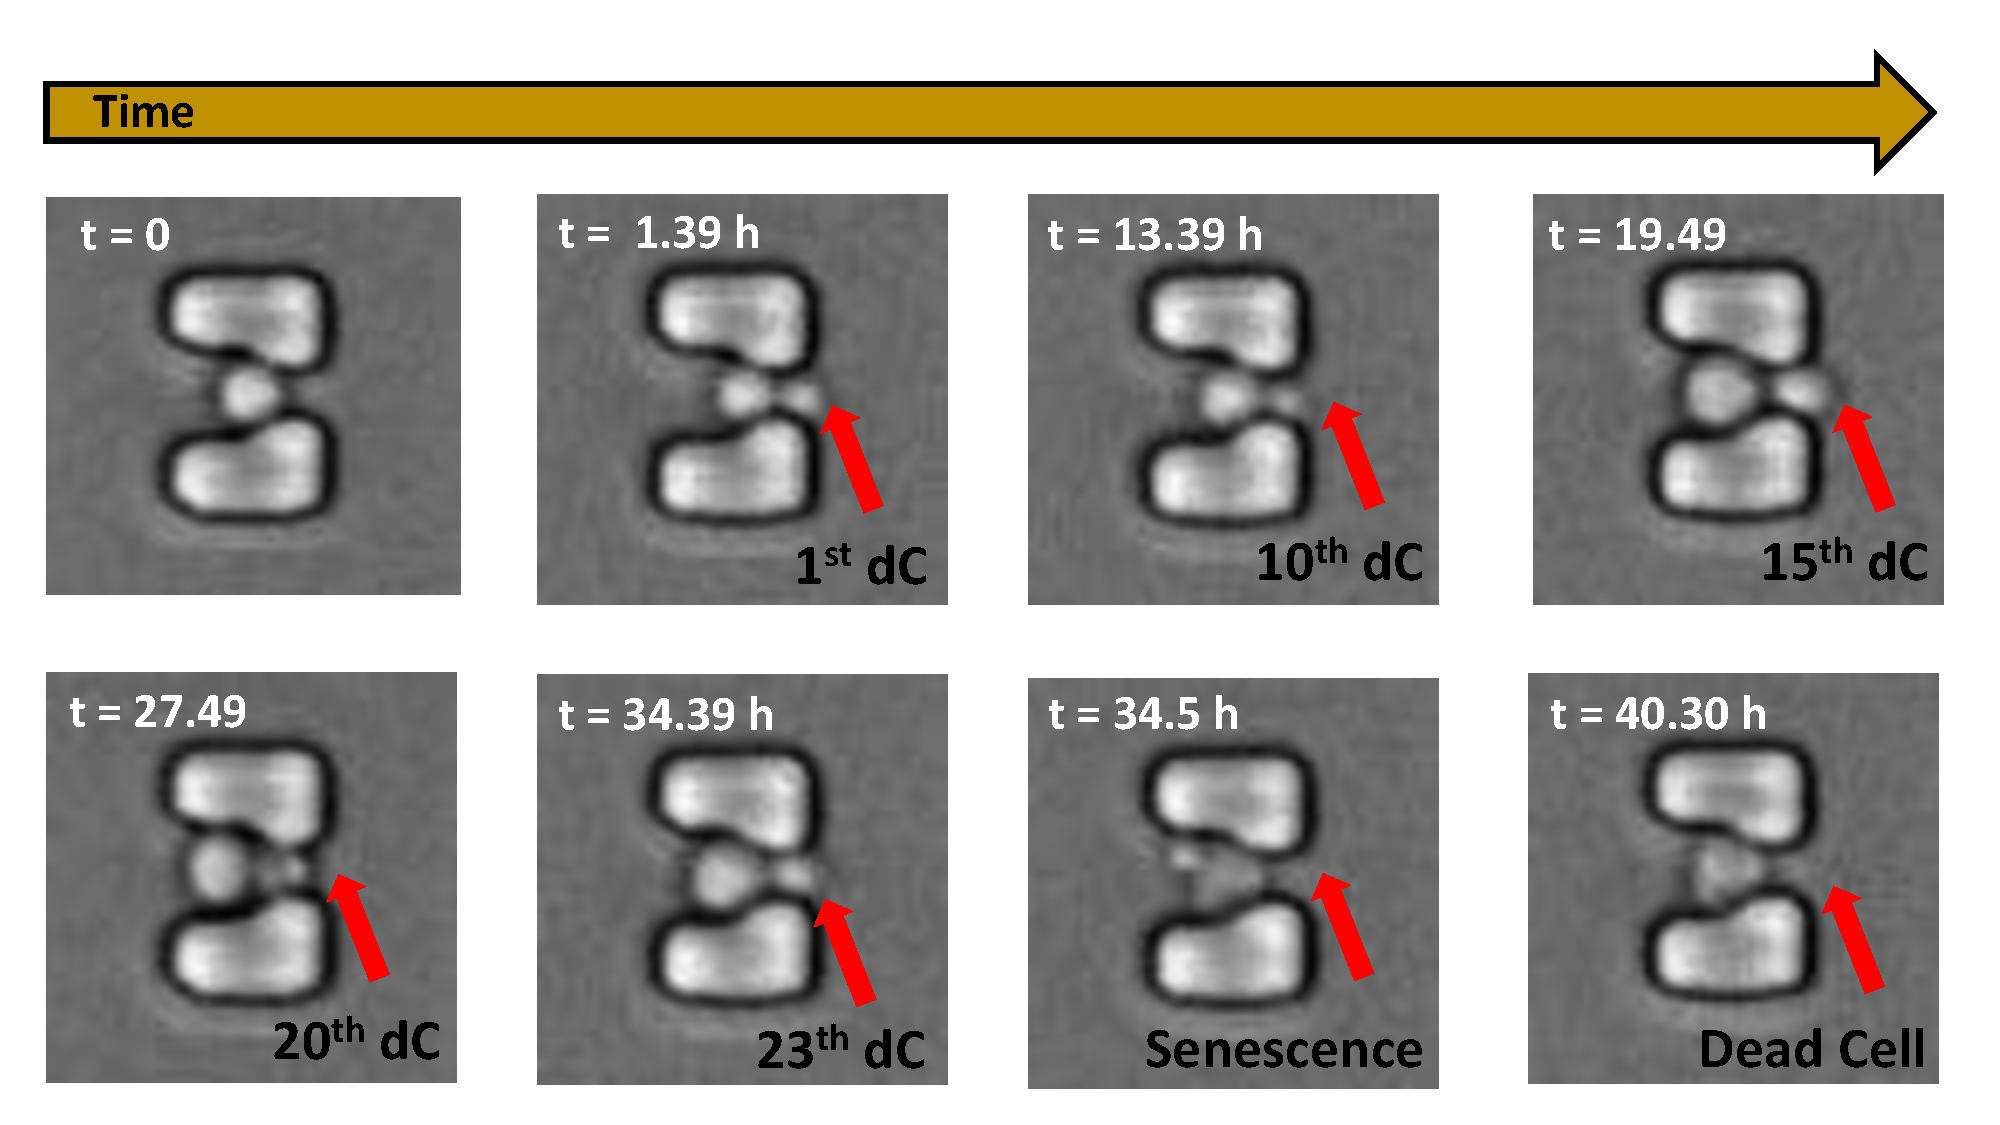
\includegraphics[width=\textwidth,height=10 cm]{Patterns/cellSteps.pdf}
% \caption{ An example of time-lapse microfluidics images.}
% \label{fig:imageData}
% \end{figure*}

 
% \begin{figure*}
% \centering
% 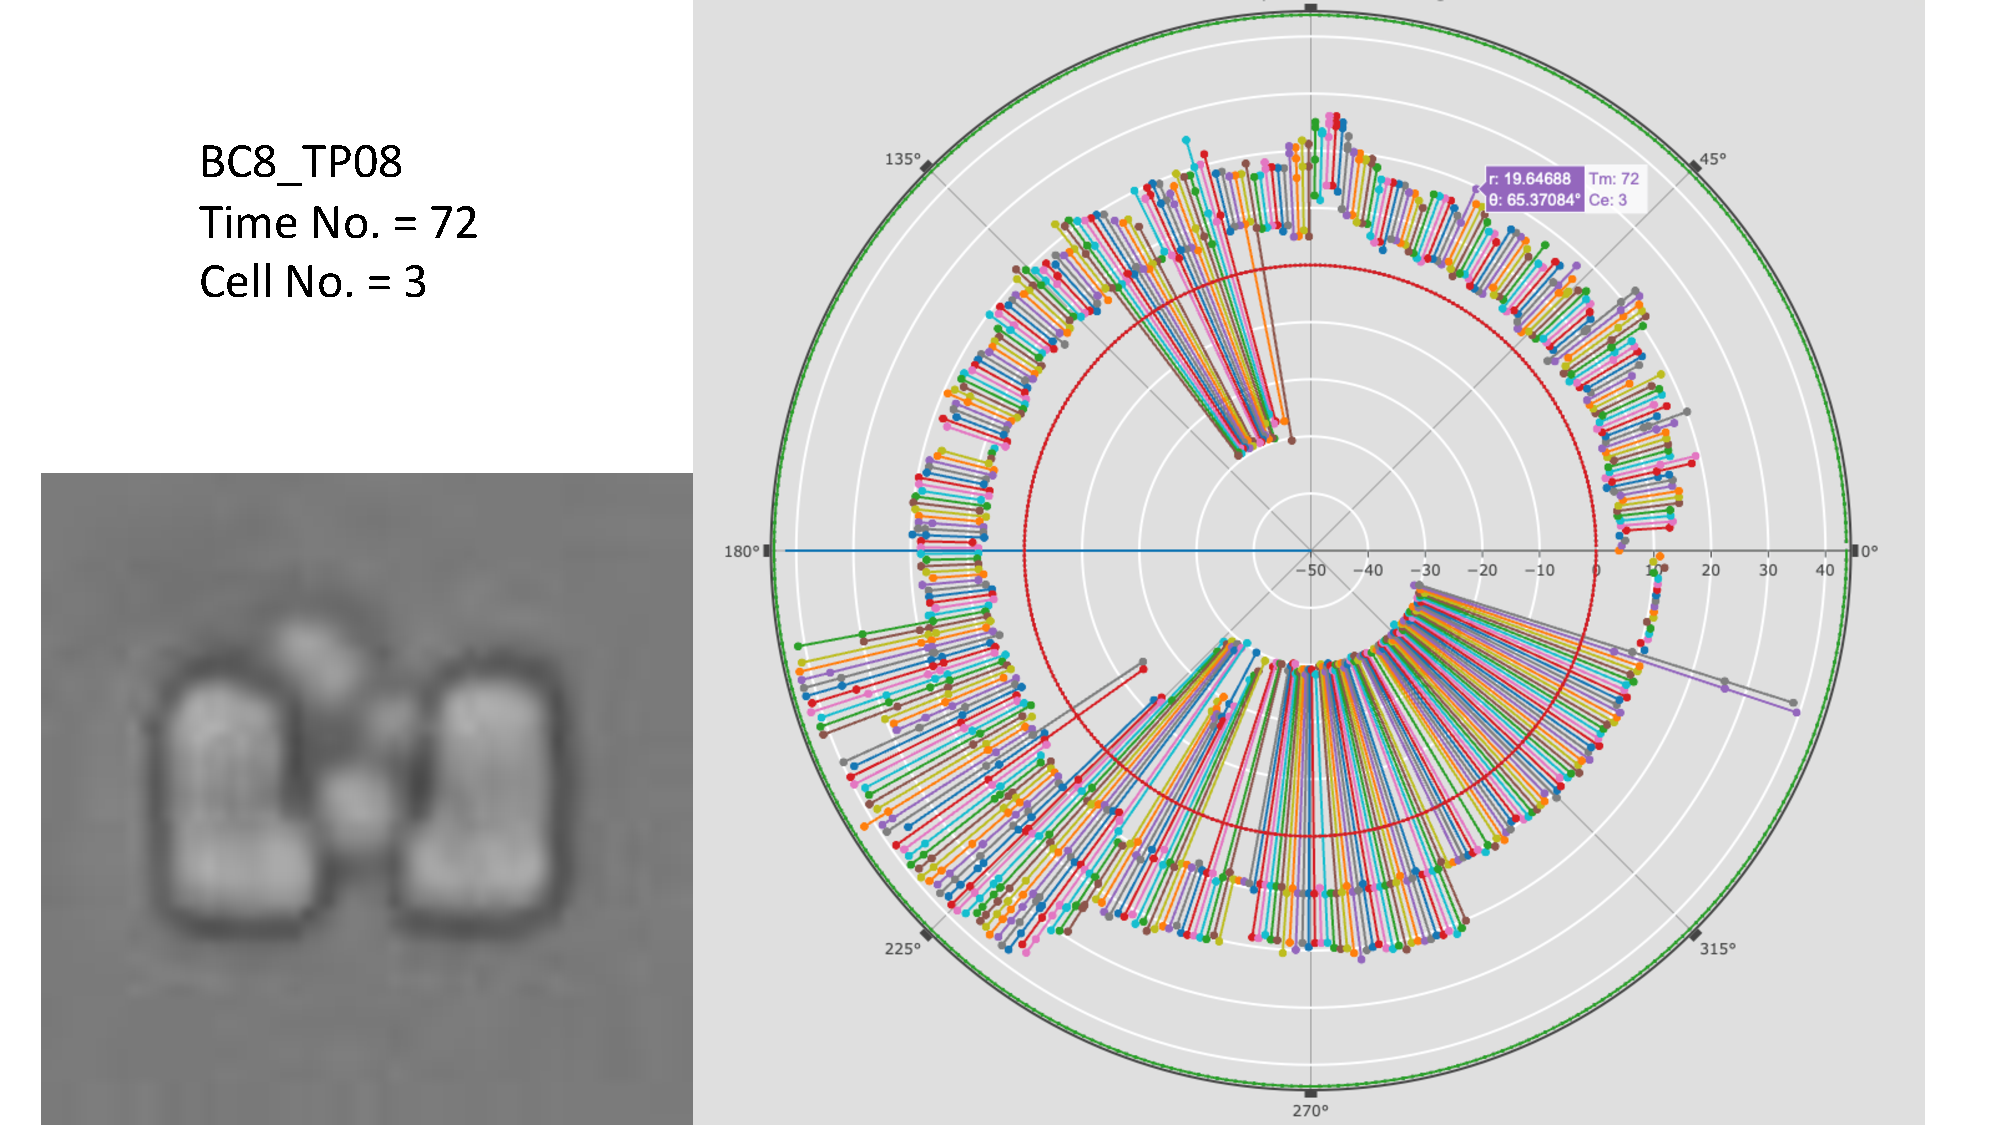
\includegraphics[width=\textwidth,height=10 cm]{Patterns/bc8_tp8.pdf}
% \caption{ An example of time-lapse microfluidics image (Beacon08 Trap08).}
% \label{fig:imageData}
% \end{figure*}


% \begin{figure*}
% \centering
% 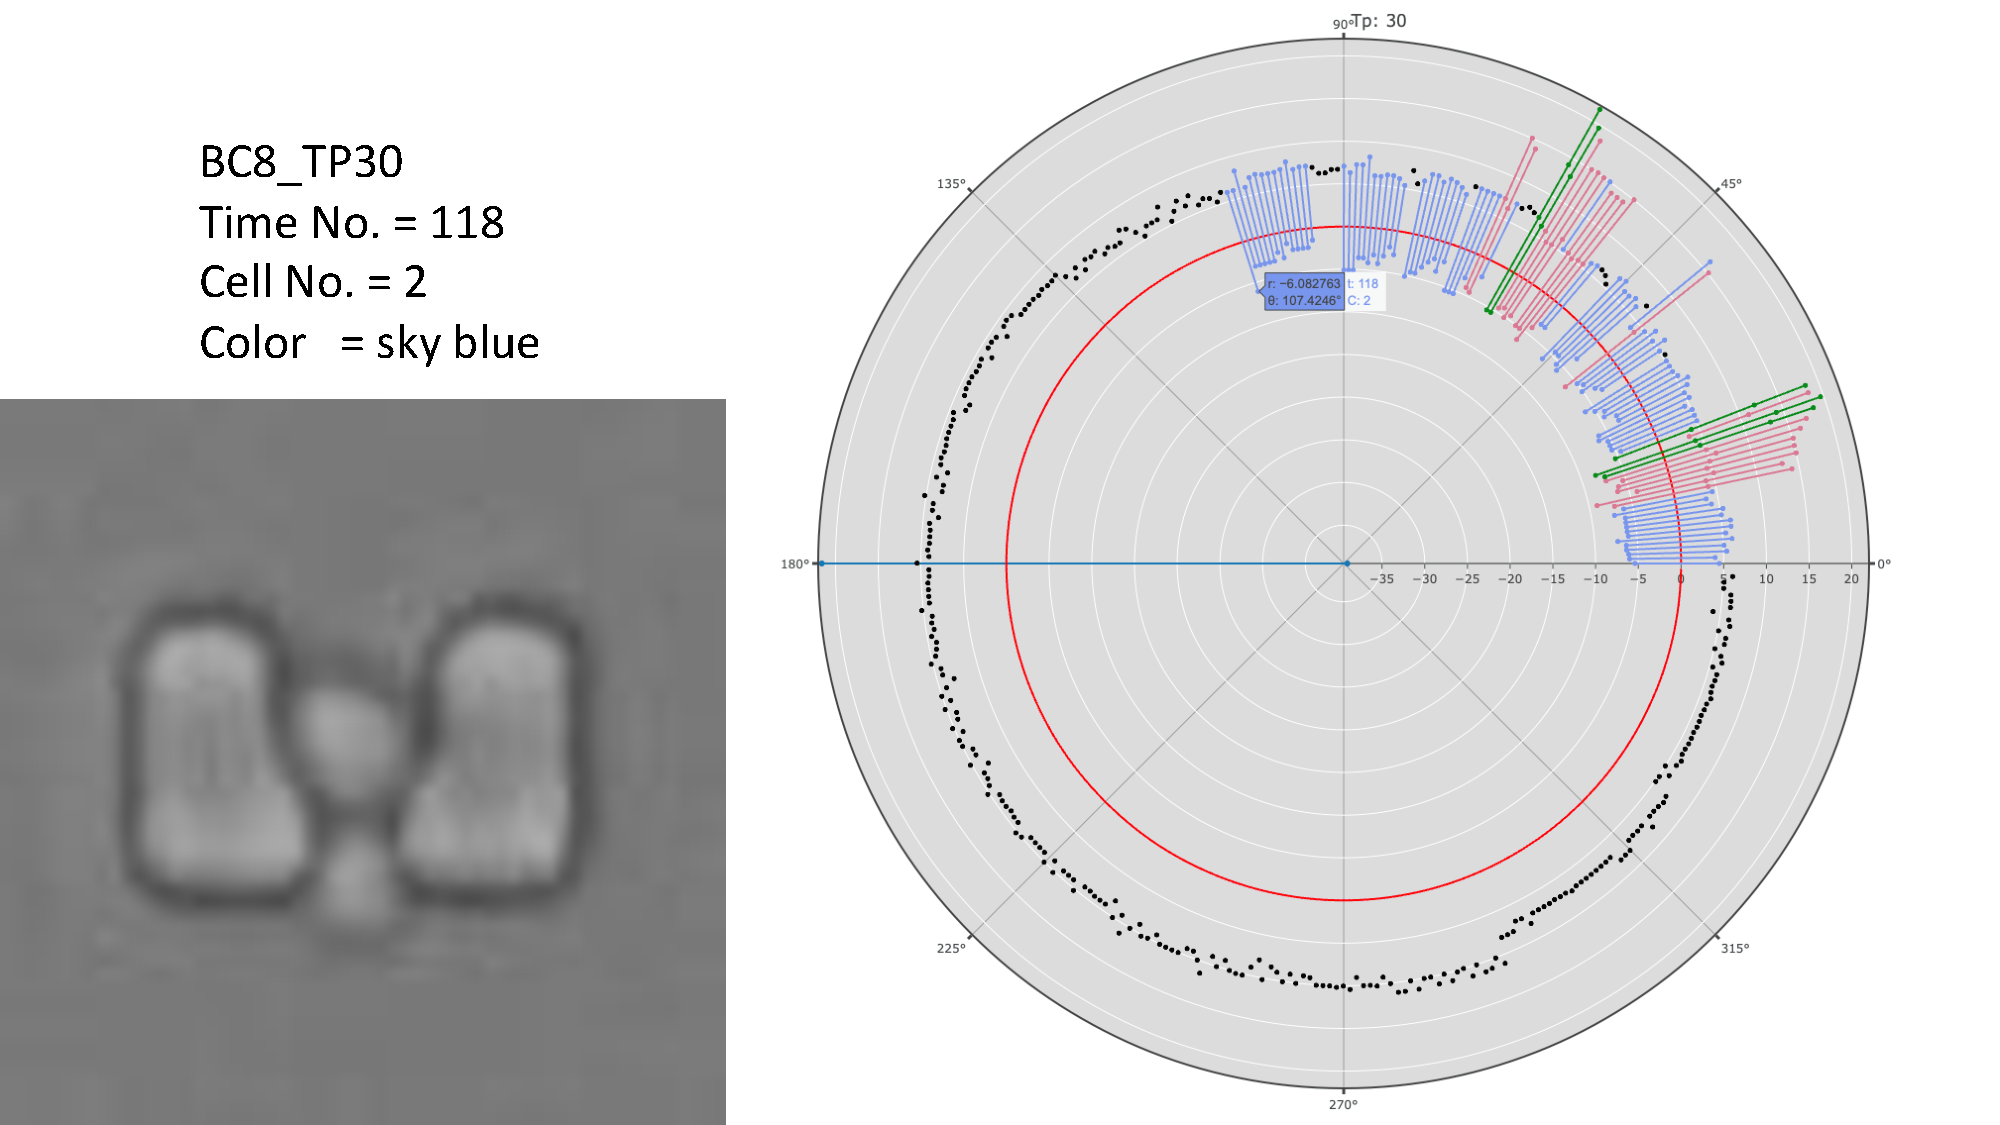
\includegraphics[width=\textwidth,height=10 cm]{Patterns/bc8_tp30.pdf}
% \caption{ An example of time-lapse microfluidics images (Beacon08 Trap30).}
% \label{fig:imageData}
% \end{figure*}


% \begin{figure*}
% \centering
% 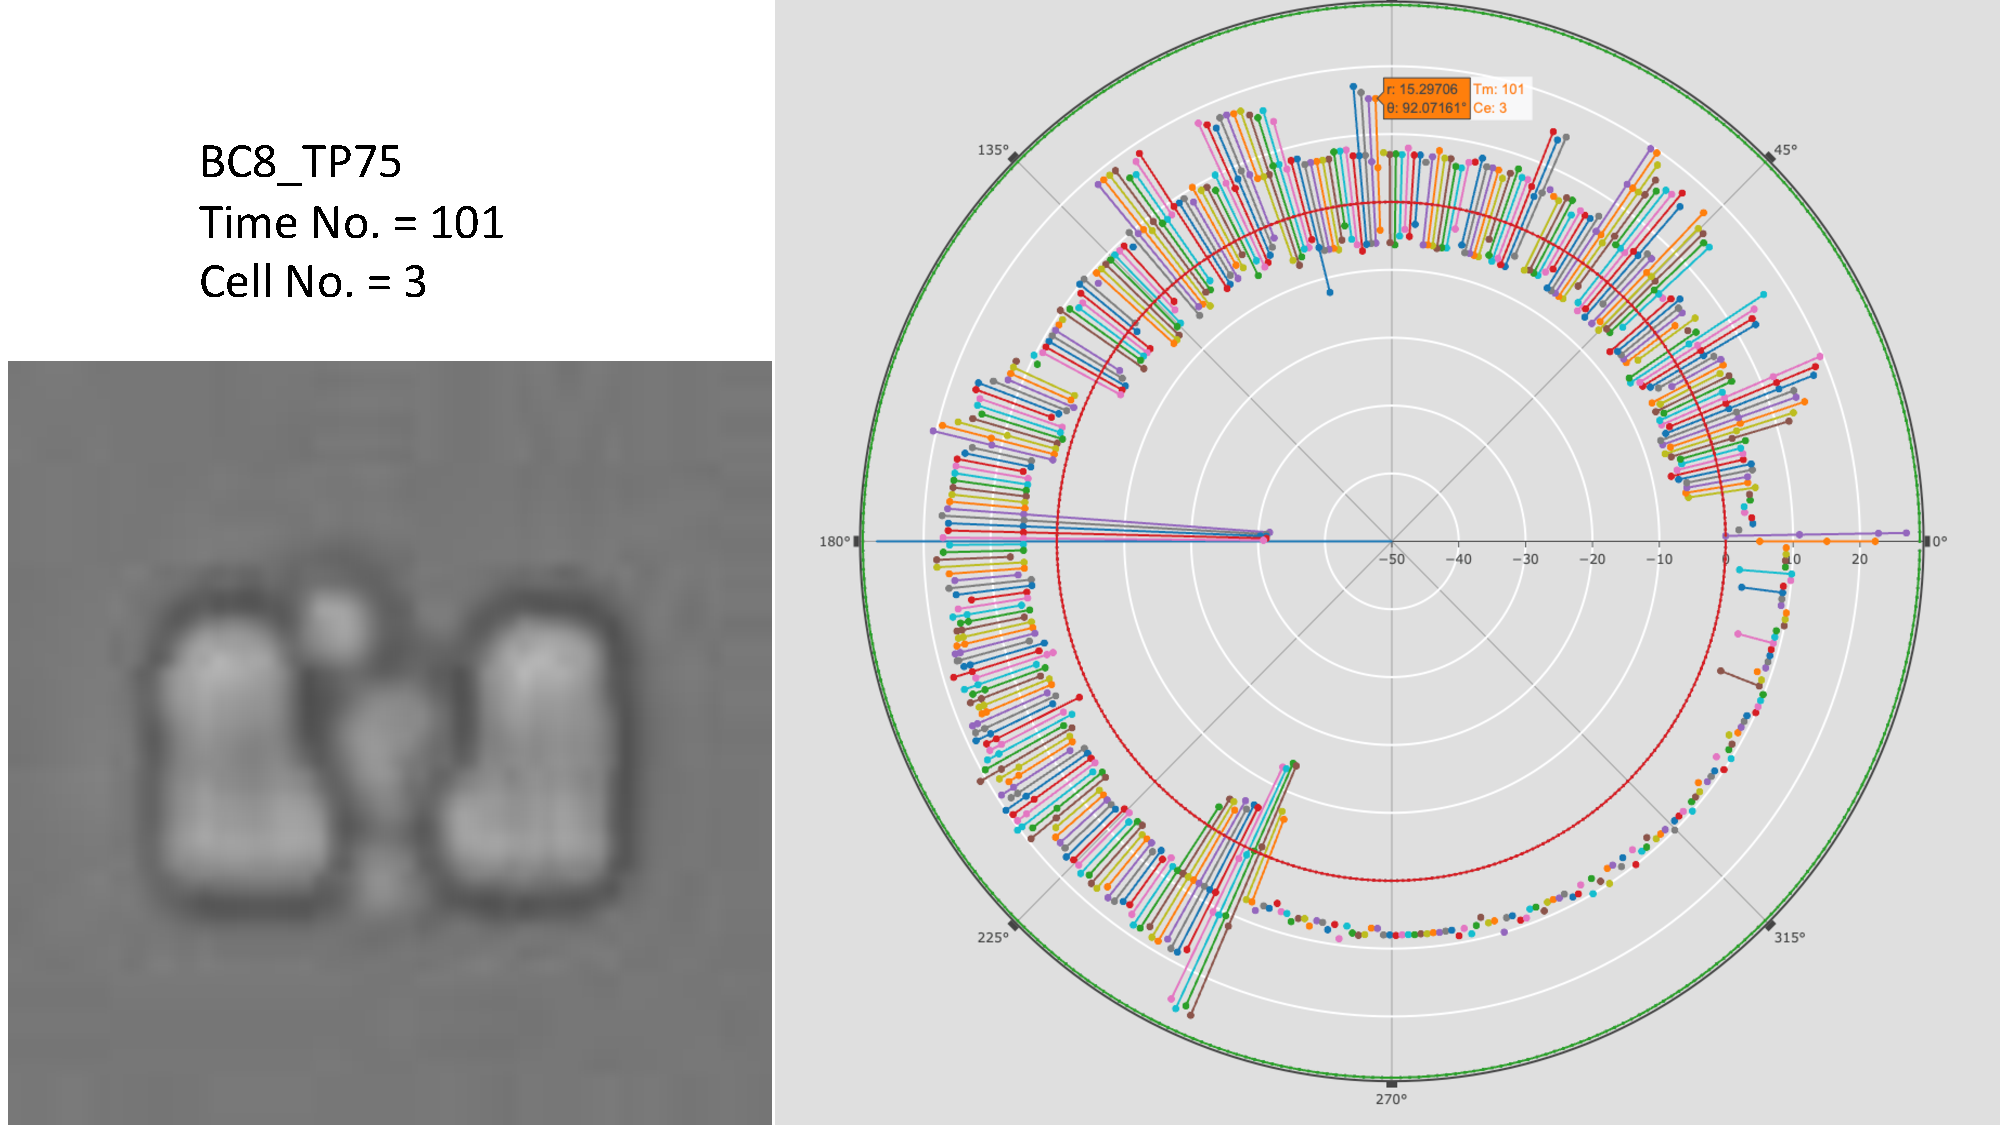
\includegraphics[width=\textwidth,height=10 cm]{Patterns/bc8_tp75.pdf}
% \caption{ An example of time-lapse microfluidics images (Beacon08 Trap75).}
% \label{fig:imageData}
% \end{figure*}


% \begin{figure*}
% \centering
% 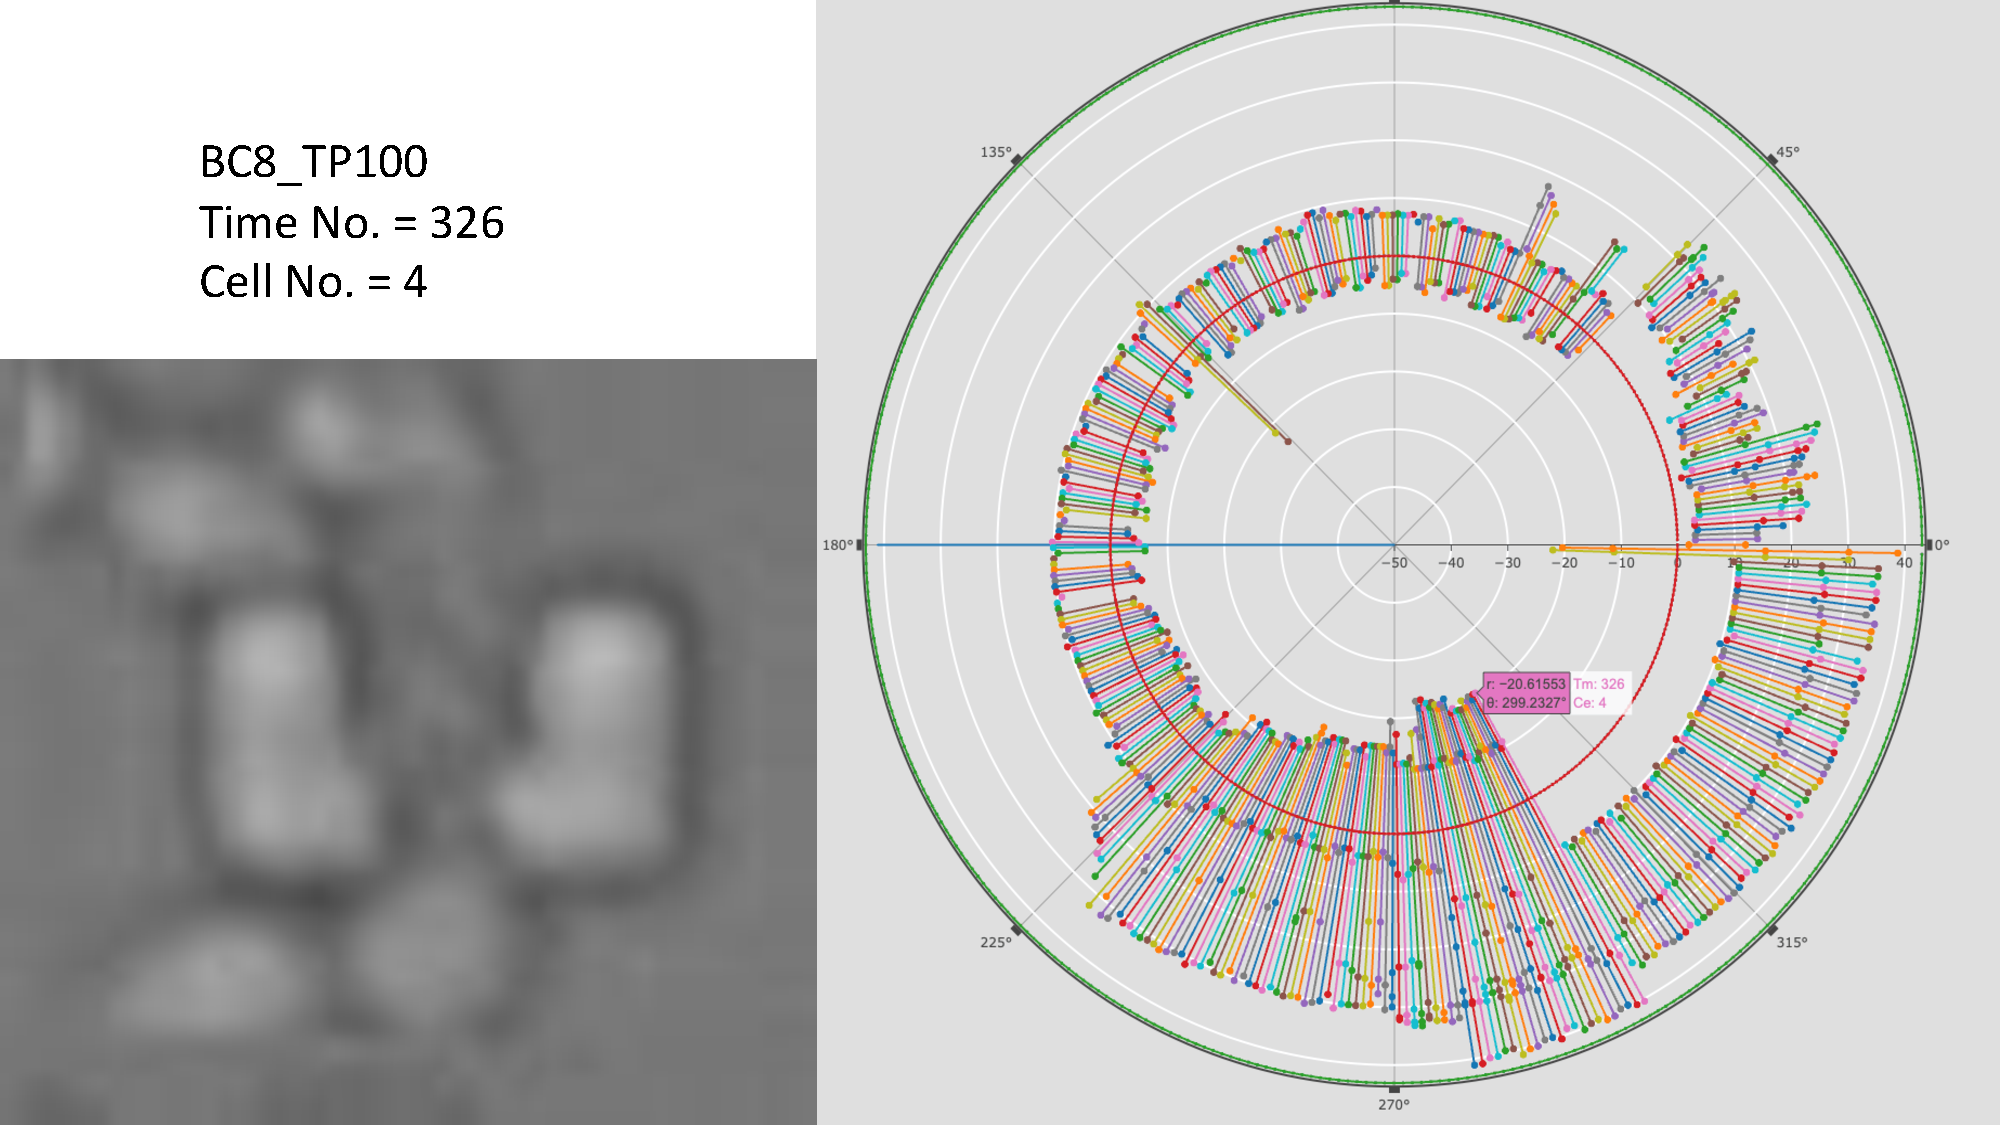
\includegraphics[width=\textwidth,height=10 cm]{Patterns/bc8_tp100.pdf}
% \caption{ An example of time-lapse microfluidics images (Beacon08 Trap100).}
% \label{fig:imageData}
% \end{figure*}


\section{Supplemental Information}

\paragraph*{S1 Fig.}
\label{S1_Fig}
{\bf  Cell distance calculation method.} (a) trap reference point. (b) an example of cell distance from reference point. (c) Sample of some images with labeled cells. 



\begin{figure*}
\centering
\includegraphics[width=\textwidth,height=10 cm]{Patterns/compare.pdf}
\caption{  $\mu$Polar visualization for several traps from microfluidics images.}
\label{fig:compare}
\end{figure*}



\paragraph*{S1 Table.}

\label{S1_Table}
{\bf Grid search and augmentation options.} A total of 108 combinations were trained without and with augmented dataset. 


\subsection*{Acknowledgment}

The work is partially supported by the NSF CAREER award \#1453078 (transferred to \#1720215), NSF award \#1761839, a  start-up fund, internal CEACSE awards from the University of Tennessee at Chattanooga, and the computing facility of the SimCenter at the University of Tennessee at Chattanooga. We also acknowledge the support of NIH grants \#R01AG052507 and \#R42AG058368.


\subsection*{Author contributions}


\subsection*{Declaration on interests}

The authors declare no competing interests.  

\begin{thebibliography}{00}

\bibitem{r1}

CARPENTERA. E.: Image-based chemical screening.NatureChemical Biology 3, 8 (2007), 461–465


\bibitem{r2}
WOLLMANR., STUURMANN.: High throughput microscopy:From raw images to discoveries.Journal of Cell Science 120,21(2007), 3715–3722

\bibitem{r2.6}
Oates, A. C., Gorfinkiel, N., Gonzalez-Gaitan, M. & Heisenberg, C.-P. Quantitative approaches in developmental biology. Nat. Rev. Genet. 10, 517–530 (2009).



\bibitem{r2.7}
Amat, F. et al. Fast, accurate reconstruction of cell lineages from large-scale fluorescence microscopy data. Nat. Methods 11, 951–958 (2014).

\bibitem{r2.8}
Mavrakis, M., Rikhy, R., Lilly, M. & Lippincott-Schwartz, J. Fluorescence imaging techniques for studying Drosophila embryo development. Curr. Protoc. Cell Biol. 39, 4.18.1–4.18.43 (2008).

\bibitem{r2.9}
Buckingham, M. E. & Meilhac, S. M. Tracing cells for tracking cell lineage and clonal behavior. Dev. Cell 21, 394–409 (2011).

\bibitem{r2.10}
Olivier, N. et al. Cell lineage reconstruction of early zebrafish embryos using label-free nonlinear microscopy. Science 329, 967–971 (2010).


\bibitem{r2.2}
Farokhi H, Ghayesh MH (2018) Nonlinear mechanics of electrically actuated microplates. International Journal of Engineering Science 123: 197-213.

\bibitem{r2.1}
Ghayesh MH (2018) Mechanics of tapered AFG shear-deformable microbeams. Microsystem Technologies 24(4): 1743-1754.


\bibitem{r2.3}
Şimşek M (2016) Nonlinear free vibration of a functionally graded nanobeam using nonlocal strain gradient theory and a novel Hamiltonian approach. International Journal of Engineering Science 105: 12-27.

\bibitem{r2.4}
 Bhagat AAS, Bow H, Hou HW, Tan SJ, Han J, et al. (2010) Microfluidics for cell separation. Med Biol Eng Compu 48: 999-1014.

\bibitem{r2.5}
Shafiee H, Jahangir M, Inci F, Wang S, Willenbrecht RB, et al. (2013) Acute on-chip HIV detection through label-free electrical sensing of viral nano- lysate. Small 9(15): 2553-2563.




\bibitem{r3}
JENSENE. C.: Overview of live-cell imaging: Require-ments and methods used.The Anatomical Record 296, 1 (2013),1–8

\bibitem{ref01}

V. Longo, G. Shadel, M. Kaeberlein and B.  Kennedy, Replicative and Chronological Aging in Saccharomyces cerevisiae, Cell Metabolism, 2002,16(1):18-31.




\bibitem{ref02}
R. Eilsand and C. Athale, Computational imaging in cell biology, Cell Biol.2003, 16: 477-48.

\bibitem{ref02.2}
M. Ghafari,  et al. , Prototyping a family tree algorithm to estimate yeast replicative lifespan from time-lapse microfluidic images, IEEESouthEastConf. 2020, (awaiting for publication)



\bibitem{ref03}
D. Webb and A. Horwitz, New dimensions in cell migration, Cell Biol, 2003,  5: 690-692.

% \bibitem{ref04}
% M. Kaeberlein, K. Kirkland, S. Fields and B. Kennedy, Sir2-Independent Life Span Extension by Calorie Restriction in Yeast, PLoS Biology,,2004, 2(9):e296.

\bibitem{ref4.2}
H. Qin, Estimating network changes from lifespan measurements using a parsimonious gene network model of cellular aging, BMC Bioinformatics 20, 599 ,2019, doi:10.1186/s12859-019-3177-7









\bibitem{ref05}
H. Tsai et .al, Usiigaci: Instance-aware cell tracking in stain-free phase contrast microscopy enabled by machine learnin. 2019, doi.org/10.1016/j.softx.2019.02.007.

\bibi



tem{ref07}

D. Botstein and G. Fink, Yeast: An experimental organism for 21st Century biology. Genetics, 2001, 189(3): 695-704.


\bibitem{ref08}

K. Steffen, B. Kennedy and M Kaeberlein, Measuring replicative life span in the budding yeast, JoVE, 2009,  28: 1-5.

\bibitem{ref09}

M. Kaeberlein and B. Kennedy, Large-scale identification in yeast of conserved ageing genes. Mech Ageing Dev,2005, 126(1):17-21.

\bibitem{ref10}

D. Sinclair, K. Mills, and L. Guarente,  Aging in Saccharomyces cerevisiae, Annu. Rev,  Microbiol, 1998, 52: 533-560.


\bibitem{ref11}

S. Enfors  et al. , Physiological responses to mixing in large scale bioreactors, J Biotechnol,2001, 85: 175-185


\bibitem{ref12}

K. Chen, M. Crane and  M. Kaeberlein, microfluidics Technologies for Yeast Replicative Lifespan Studies. Mechanisms of ageing and development, 2017, 161(Pt B):262-269.


\bibitem{ref13}

 M. Jo, W. Liu, L. Gu, W. Dang and  L. Qin, High-throughput analysis of yeast replicative aging using a microfluidics system, Proc. Nati. Acad. Sci. USA, 2015, 112: 9364-9369.


\bibitem{ref14}

M. McCormick,  J.Delaney, M. Tsuchiya, et alA comprehensive analysis of replicative lifespan in 4,698 single-gene deletion strains uncovers conserved mechanisms of aging, Cell metabolism, 2015, 22(5):895-906.


\bibitem{ref15}
S. Pang,  et al. ,A novel YOLOv3-arch model for identifying cholelithiasis and classifying gallstones on CT images, PLoS ONE, 2019, 14(6): e0217647. https://doi.org/10.1371/journal. pone.021764

\bibitem{ref16}
C.  Laura, P. Hofmann, K. Drechselr  and S. Wesarg, Automatic detection of the nasal cavities and paranasal sinuses using deep neural networks, In IEEE 16th International Symposium on Biomedical Imaging,2019, pages 1154–1157. IEEE.

\bibitem{ref17}
J. Martin, et al., The impact of 2D cine MR imaging parameters on automated tumor and organ localization for MR-guided real-time adaptive radiotherapy. Physics in Medicine and Biology, 2018, 63(23):235005.

\bibitem{ref18}
S. Ramachandran, J. George, S. Skaria, and  V. Varun,  Using YOLO based deep learning network for real time detection and localization of lung nodules from low dose CT scans, In Kensaku Mori and Nicholas Petrick, editors, Medical Imaging 2018: Computer-Aided Diagnosis, 2018, volume 10575, page 53. SPIE.

\bibitem{ref19}
J. Redmon and A. Farhadi. YOLOv3: An Incremental Improvement. Technical report, University of Washington, 2018.

\bibitem{ref20}
Z. Zhao, P. Zheng, S. Xu, and X Wu, Object Detection With Deep Learning: A Review. IEEE Transactions on Neural Networks and Learning Systems, 2019, pages 1–21.


\end{thebibliography}



% We provide a concise description of live cell imaging in Section 
% 2. Next, in Section 
% 3, we describe our analytical approach. Based on this, Section 
% 4 contains the results of a systematic analysis of visualization methods cell imaging. 
% This includes reports on domain and data characterization (Section 4.1),
% task abstraction (Section 4.2), and
% visual encoding and interaction design (Section 4.3).
% We discuss the implications of our analysis,including a number of research gaps, in Section 5
% conclude with Section 6.


%https://www.osti.gov/servlets/purl/1557948
%https://onlinelibrary.wiley.com/doi/epdf/10.1111/cgf.12784



% Imaging of fluorescently labeled proteins in living cells provides spatial and temporal information on their subcellular localization. This is essential to understand their role in dynamic processes such as cell division. In addition, time-lapse microscopy allows direct analysis of the correlation (or lack thereof) between distinct events at the single cell level, which could be masked in bulk population studies such as time-courses of synchronized cultures. Such correlations might reveal functional relationships, coordination of events in space and time, and feedback regulatory loops (see [1] for a detailed discussion of these topics).
% In budding yeast cells, the site of cytokinesis (termed the bud neck) is marked by the presence of a membrane-associated, septin- based collar [2]. Cytokinesis begins at the end of mitosis when the septin collar splits into two rings, defining a compartment where actomyosin ring contraction takes place [3]. Closure of this con- tractile ring and septum deposition drive the overlying plasma membrane inward, in a process akin to furrow ingression in animal cells (see [4, 5] for reviews). The ring then disassembles, allowing fission of the contracted membrane, in a process termed abscission [3]. After completion of cytokinesis, cell wall degradation at the septation site allows separation of mother and daughter cells [6]. Here, we describe optimized methods to image multiple cytokinesis events in living yeast cells, namely septin ring dynamics, acto- myosin ring contraction, and plasma membrane ingression at the mother–bud neck.

% Time-lapse imaging files are relatively large and it is therefore useful to ensure that enough memory space and computer processing power are available to process them (each of the image fields in the above example represent 1200 [20×60] frames for each channel, between 0.5 and 1.5 GB in size).

%https://link.springer.com/content/pdf/10.1007%2F978-1-4939-3145-3.pdf














\end{document}
